% !TEX root = diplomarbeit.tex
\chapter{Digitale Speisekarte}
\renewcommand{\kapitelautor}{Autor: Katharina Joksch}

%%%%%%%%%%%%%%%%%%%%%%%%%%%%%%%%%%%%%%%%%%%%%%%%%%%%%%%%%%%%%%%%%%%%%%%%%%%%%%%
\section{Allgemeine technische Planung}

  \subsection{PhpStorm}

PhpStorm ist eine PHP Entwicklungsumgebung der Firma JetBrains. Die tschechische Firma JetBrains wurde 2000 gegründet und legt ihren Fokus auf die Entwicklung von IDEs. Davon kann in PhpStorm enorm profitiert werden, denn diese IDE punktet nicht nur durch ihre Geschwindigkeit sondern auch durch die Möglichkeit sie nahezu komplett an die eigenen Programmierbedürfnisse anpassen zu können. Natürlich ermöglicht sie wie die meisten Entwicklungsumgebungen auch die Autovervollständigung des Codes, während der Eingabe von Befehlen. PhpStorm zeigt den Code dank Syntax-Highlightning übersichtlich an und stellt das Ordnerverzeichnis der Projekte strukturiert in einem Fenster daneben an. Diese Eigenschaft unterstützt das Arbeiten mit Frameworks, weswegen diese IDE für die Entwicklung der digitalen Speisekarte verwendet wurde.

  \subsection{Zusammenspiel der Komponenten}

Die Webapplikation baut, wie folgende Abbildung aufweist, auf mehreren Komponenten auf, um eine optimale Performance zu gewährleisten.
Die Applikation, also die digitale Speisekarte und das Admininterface, wurden in der Entwicklungsumgebung PhpStorm programmiert, da diese einen guten Überblick über die Ordnerstruktur bietet.
Sie wurde mit dem Framework Symfony 2.7 entwickelt, welches in Model, View und Controller unterteilt, damit durchgehend eine ordentliche Struktur beibehalten werden kann. In der Model Schicht wurde mit dem Framework Doctrine gearbeitet um die Daten objektrelational behandeln zu können. Auf dieser Ebene wird mit der Datenbank, wofür MySQL gewählt wurde, kommuniziert.
Der Controller dient als Schnittstelle für Model und View. Er leitet die Daten zwischen diesen zwei Schichten hin und her.
Die View-Ebene dient dazu die Daten visuell darzustellen. Dadurch können die Speisekarte und der Adminbereich im Frontend aufgerufen werden. Da es einfacher ist Daten vom Controller mit einer Template Engine aufzurufen, wurde in dieser Schicht mit Twig gearbeitet. Um das Layout responsive darzustellen und somit auf jede Gerätegröße anzupassen, wurde mit Bootstrap 4 alpha gearbeitet. Mithilfe von Sass konnten die vordefinierten Bootstrapvariablen verändert und dadurch das Layout mit wenig Aufwand komplett an die eigenen Wünsche angepasst werden.
Um die dadurch entstandene Sass-Datei in den Twig beziehungsungsweise HTML-Dateien einbinden zu können wurde sie mithilfe des Task-Runners Gulp kompiliert.\\
			\begin{figure}[H]
			\begin{centering}
			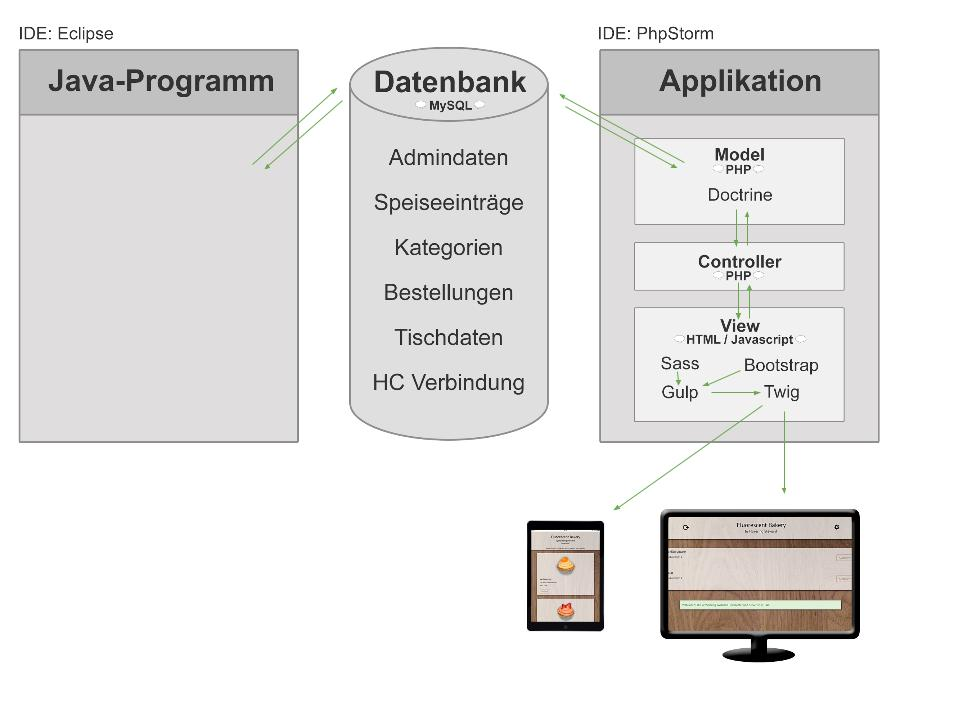
\includegraphics[width = 1\textwidth]{Bilder/Jok_zusammenspiel_applikation.jpg}
			\par\end{centering}
			\caption{Zusammenspiel der Komponenten}
			\label{Zusammenspiel der Komponenten}
			\end{figure}

%%%%%%%%%%%%%%%%%%%%%%%%%%%%%%%%%%%%%%%%%%%%%%%%%%%%%%%%%%%%%%%%%%%%%%%%%%%%%%%
\section{Backend}

  \subsection{Technische Planung}

    \subsubsection{Apache HTTP Server}

Der {Apache HTTP Server\cite{apachehttpserver}} ist eine freie Software, welche von der Apache Software Foundation entwickelt wurde. Der Apache Webserver kann mit den Betriebsystemen Linux, Unix, Windows, Mac OS X, Betware und OpenBSD arbeiten. Dieser Server ermöglicht es Webseiten als http-Services bereitzustellen, damit sie anschließend in Web-Browsern aufgerufen werden können.

    \subsubsection{MAMP und XAMPP}

{MAMP\cite{mamp}} und {XAMPP\cite{xampp}} sind Pakete, welche freie Software enthalten, die dazu dient dynamische Webseiten zur Verfügung zu stellen. Unter dynamischen Webseiten versteht man, Seiten die auf Funktionen im Backend zugreifen und mithilfe welcher Inhalte meist erst im Moment der Anfrage erzeugt werden, wodurch sie aktuell gehalten werden können.
\begin{itemize}
    \item \textbf{MAMP}\\
MAMP besteht aus dem My Apache Webserver, dem Datenbanksystem MySQL und den PHP Versionen 5.1.6 und 5.5.9. Dadurch ergibt sich auch die Bezeichnung dieses Softwarepakets, da es sich aus den Anfangsbuchstaben der verwendeten Komponenten zusammenstellt. Außerdem beinhaltet es eine aktuelle {Python\cite{python}} Version, welche als objektorientierte Programmiersprache dazu dient schneller Programme zu entwickeln, als es mit sämtlichen anderen Programmiersprachen möglich ist. Zusätzlich kann in dem Paket auch mit der Programmiersprache {Perl\cite{perl}}, welche in erster Linie bei der Verwaltung von Textdateien behilflich ist. MAMP ist unter der "{GNU\cite{gnu}} (General Public License)" lizenziert, was bedeutet, dass es frei verändert und verbreitet werden darf. Das Paket wird von den Betriebssystemen Windows und OS X unterstützt.
    \item \textbf{XAMPP}\\
Das XAMPP-Paket wird aus dem Apache HTTP Server, der Datenbank MariaDB, welche auf den Grundlagen der MySQL Datenbank beruht, und den Programmiersprachen PHP und Perl. Das "X" am Anfang der Bezeichnung des Pakets, steht für die vielen Betriebssysteme, welche damit arbeiten können. XAMPP ist kompatibel mit Windows, OS X, Linux und Solaris. Dieses Paket ist ebenfalls unter der "GNU"-Lizenz freigegeben.
  \end{itemize}
Sowohl MAMP als auch XAMPP bieten daher effiziente Pakete, welche beim Entwickeln von dynamischen Webseiten sehr zu empfehlen sind. Für die Erstellung der digitalen Speisekarte fiel die Entscheidung letztendlich auf MAMP, da nur auf den Betriebssystemen Windows und OS X entwickelt wurde. Außerdem ist das Interface dieses Pakets einfacher gehalten und dadurch übersichtlicher für den Anwender. Ein weiterer Vorteil von MAMP ist, dass auf dem Startverzeichnis unter den Einstellungen ein favorisierter Link gespeichert werden konnte, welcher daraufhin auf der Startseite aufgerufen werden kann. Diese Eigenschaft ermöglichte es die digitale Speisekarte schneller aufzurufen.

    \subsubsection{Doctrine}

{Doctrine\cite{doctrine}} ist ein Framework, welches dabei hilft ein objektrelationales Abbild zu erschaffen. Bei objektrelationalen Abbildungen werden Tabellen wie Klassen und Tabellenzeilen wie Objekte behandelt. Das vereinfacht den Zugriff auf verschiedene Datenbanken im Vergleich zu dem Zugriff mittels Plain PHP um ein Vielfaches.

    \subsubsection{Symfony}

Da Frameworks, welche auf dem Model-View-Controller Schema beruhen, den Arbeitsaufwand erleichtern und dafür sorgen, dass während des Programmierens eine ordentliche Struktur im Code beibehalten wird, wurde eines als Grundgerüst für die Entwicklung der Applikation verwendet. Nachdem eine Speisekarte viele Informationen enthält, welche in einer Datenbank verwaltet werden sollten, wurde ein PHP-Framework gewählt, welches den Zugriff darauf objektrelational regelt.
{Symfony\cite{symfony}} ist ein Open Source Web Application Framework, welches sowohl das Model-View-Controller Schema nützt als auch den Datenbankzugriff mittels eines objektrelationalen Abbilds regelt, weshalb es die ideale Wahl für die Umsetzung der digitalen Speisekarte und des Adminbereichs ist.
Wie bereits erwähnt, ergibt sich durch die Einteilung in Model, View und Controller während des Entwicklungsprozesses eine strukturierte Ordnung im Code.
Dies liegt daran, dass jeder dieser Schichten eine genaue Aufgabe zugeschrieben ist.
\begin{itemize}
    \item \textbf{Model(Datenhaltungsschicht)}\\
Die Model-Schicht dient dazu Daten zur Verfügung zu stellen.
    \item \textbf{View(Präsentationsschicht)}\\
In der View-Ebene werden Daten visualisiert. Diese Ebene deckt somit den Frontend Bereich der Applikation ab.
    \item \textbf{Controller(Steuerungsschicht)}\\
Der Controller fungiert als Schnittstelle zwischen der Model- und der View-Ebene. Er leitet die Daten von der Model-Schicht in die View-Schicht weiter, damit diese dort ausgegeben werden können. Außerdem nimmt er Benutzeraktionen im Frontend entgegen, wertet diese aus und behandelt sie entsprechend.
  \end{itemize}
Um diese Funktionalitäten anhand eines Szenarios zu veranschaulichen, kann auch folgendes vorgestellt werden:
Angenommen es soll ein Cupcake gebacken und im Schaufenster einer Konditorei hergezeigt werden. Dafür werden zuerst einmal Daten aus einem Rezeptbuch benötigt. Diese sind in der Model-Schicht zu finden.
Nun müssen diese Informationen jedoch noch behandelt werden um den Cupcake auch wirklich visuell erschaffen zu können. Dafür wird ein Konditor benötigt, welcher den Controller symbolisiert.
Der Konditor mischt die Zutaten zusammen, behandelt sie entsprechend indem er sie anschließend in den Ofen gibt, und stellt den Cupcake nun in dem Schaufenster seiner Konditorei, also in dem View, den Passanten zur Ansicht zur Verfügung.
			\begin{figure}[H]
			\begin{centering}
			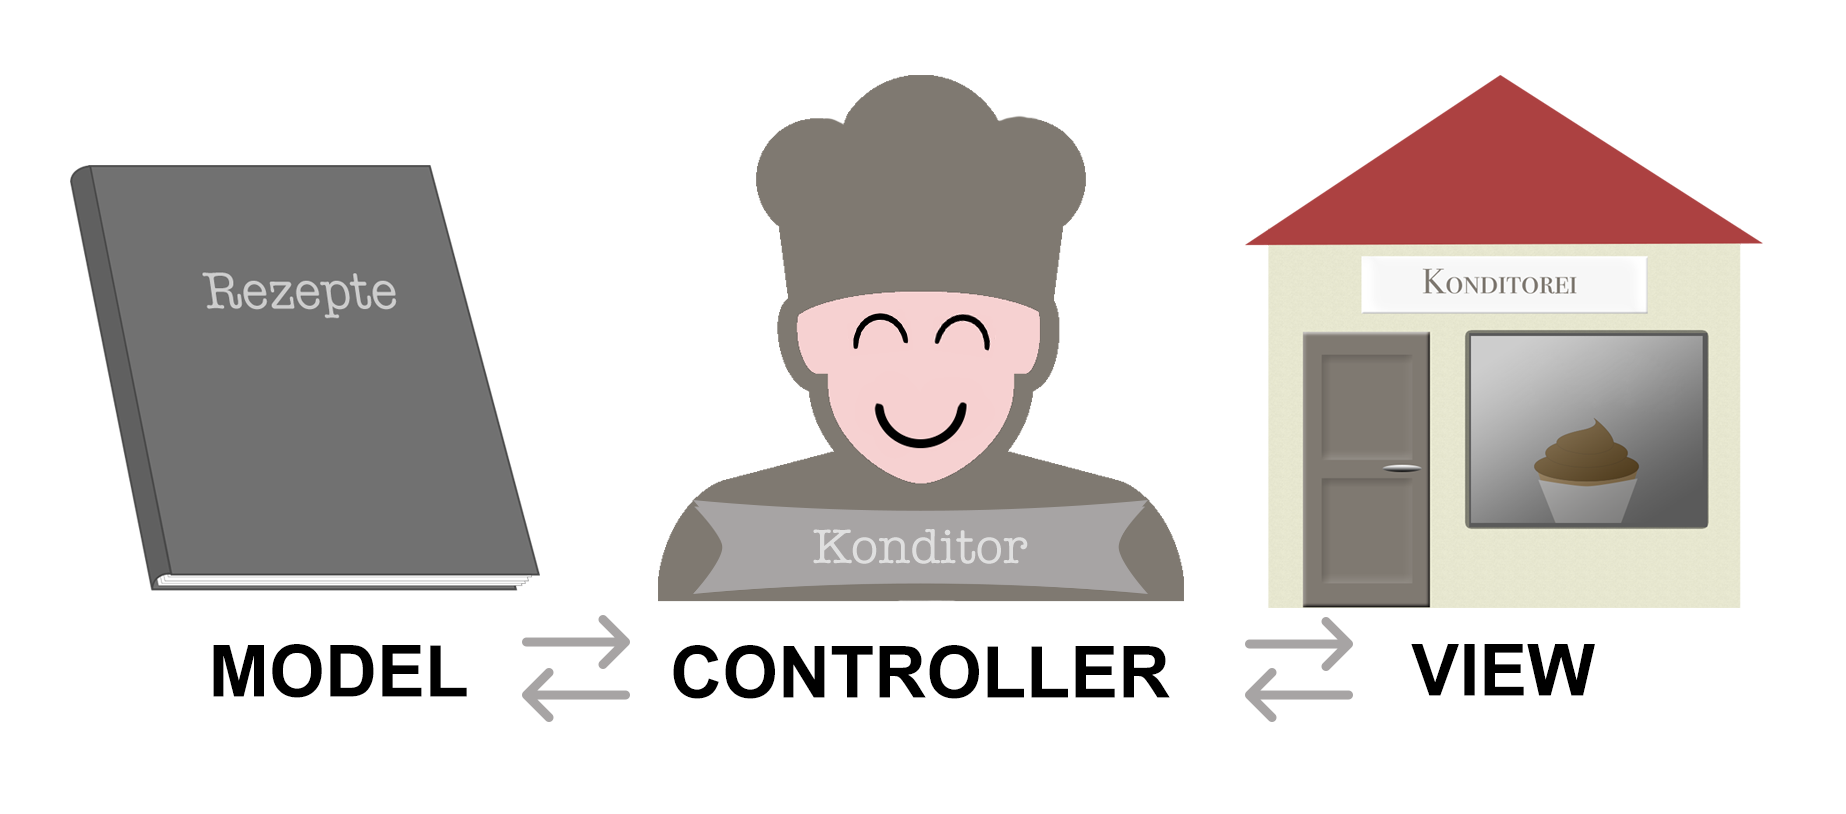
\includegraphics[width = 1\textwidth]{Bilder/Jok_mvc.png}
			\par\end{centering}
			\caption{MVC-Erklärung}
			\label{MVC-Erklärung}
			\end{figure}

    \subsubsection{ER-Modell}

Bevor die Datenbank mithilfe von Doctrine generiert wurde, wurde ein Entity Relationship Modell angefertigt um zu visualisieren wie die Tabellenverbindungen am geeignetsten aufbereitet werden können. Ein ERM dient dazu die Verknüpfungen zwischen zwei relationalen Tabellen visuell darzustellen. Die Verbindung wird dadurch gewährleistet, dass die zwei Tabellen über Foreign Keys verbunden werden, welche meist auf den Primary Key, also die ID der Tabelle, verweisen. Bei der Verknüpfung gilt es zu entscheiden ob es sich um eine ManyToMany oder um eine ManyToOne beziehungsweise OneToMany handelt. Eine ManyToMany Verbindung wird dann benötigt, wenn eine Tabelle auf viele Tabelleneinträge einer anderen Tabelle verweist und diese ebenfalls auf mehrere Einträge verlinkt. Die ManyToOne und OneToMany Verbindungsvariante wird verwendet, wenn von einem einzigen Eintrag auf mehrere einer anderen Tabelle verwiesen werden soll.
			\begin{figure}[H]
			\begin{centering}
			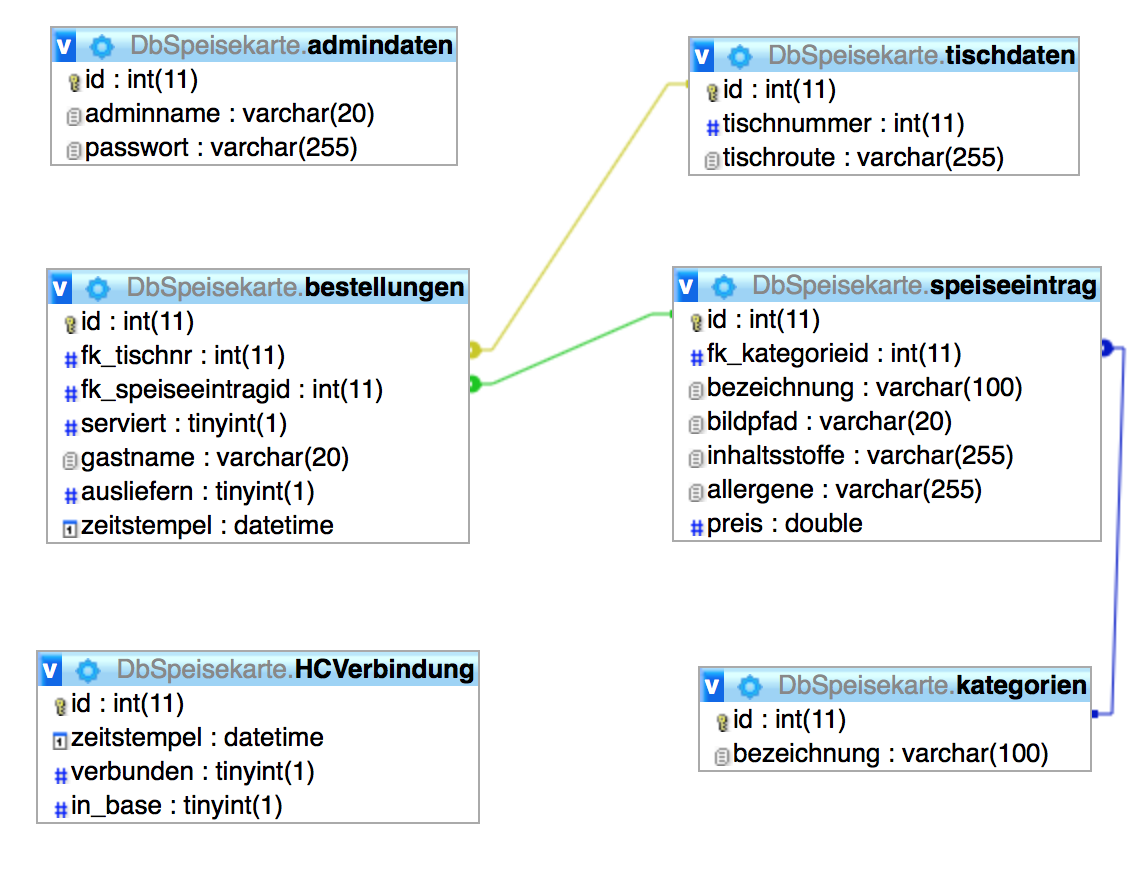
\includegraphics[width = 1\textwidth]{Bilder/Jok_ERM.png}
			\par\end{centering}
			\caption{ERM der digitalen Speisekarte}
			\label{ERM der digitalen Speisekarte}
			\end{figure}Bei der digitalen Speisekarte mussten drei Verbindungen zwischen den folgenden Tabellen erstellt werden:
\begin{itemize}
    \item \textbf{Speiseinträge und Kategorien}\\
Um den Kategorien viele Speiseeinträge zuzuweisen, musste eine ManyToOne Verknüpfung auf der Seite der Speisekarte und eine OneToMany bei den Kategorien erstellt werden. Dadurch konnte später gewährleistet werden, dass in der Speisekarte über das Menü im Header zwischen den verschiedenen Kategorien gewechselt werden kann um die ihnen zugewiesenen Speiseeinträge einsehen zu können.
    \item \textbf{Bestellungen und Speiseeinträge}\\
Damit der Administrator als auch der Gast die Möglichkeit haben zu überprüfen welche Speisen bereits bestellt wurden, war es notwendig eine ManyToOne Verbindung bei der Bestellungen-Tabelle und eine OneToMany bei der Speiseeintrag-Tabelle zu definieren. Hierbei kann ein Speiseeintrag öfters bestellt werden, weswegen die ManyToOne Verbindung auf der Seite der Bestellungen eingestellt wurde.
    \item \textbf{Bestellungen und Tischdaten}\\
Um dem Hexacopter die richtigen Tischdaten der Bestellung zukommen zu lassen, war es wichtig zwischen diesen zwei Tabellen eine Verbindung herzustellen. Da mehrere Bestellungseinträge auf dieselben Tischdaten verweisen können musste auf der Bestellungen Seite eine OneToMany und auf der Tischdaten Seite eine ManyToOne Verknüpfung erschaffen werden.
  \end{itemize}

  \subsection{Umsetzung}

    \subsubsection{Framework einrichten}

Um mit Symfony arbeiten zu können wurde zuerst der Symfony-Installer integriert. Bei einem Gerät mit dem Betriebsystem Mac OS X wurde dies durch die Eingabe folgender Befehle in das Terminal bewerkstelligt:
	\lstset{language = bash}
  	\begin{lstlisting}
sudo curl -LsS http://symfony.com/installer -o /usr/local/bin/symfony
sudo chmod a+x /usr/local/bin/symfony
  	\end{lstlisting}
Anschließend wurde ein Projekt angelegt. Dafür wurde in das Zielverzeichnis gewechselt. Um das Projekt im Anschluss über den Apache Server aufrufen zu können, empfiehlt es sich das Projekt direkt im "htdocs"-Ordner der jeweiligen LAMP Distribution abzuspeichern. Damit das Projekt auf einem Mac OS X basierenden Gerät angelegt wurde, musste der anschließende Befehl in das Terminal eingegeben werden:
	\lstset{language = bash}
  	\begin{lstlisting}
symfony new PROJEKTNAME lts
  	\end{lstlisting}
Der Befehl "lts" legt fest, dass die neueste Version von Symfony verwendet werden soll.

    \subsubsection{Seitenabrufbarkeit}

Um Seiten anzulegen, welche später im Browser angezeigt werden konnten, mussten im Controller folgende Schritte erledigt werden. Zuerst empfahl es sich Action Funktionen anzulegen. Diese wurden passend zu der jeweiligen Seite beziehungsweise zu den dementsprechenden Funktionalitäten benannt, welche im Anschluss angezeigt und ausgeführt wurden. Wenn auf der auszugebenden Seite mit einer Template Engine gearbeitet wurde, wurde als Rückgabewert der Methode der anschließende Code definiert:

	\lstset{language=php}
  	\begin{lstlisting}
$this->render('DATEIBEZEICHNUNG.html.twig')
  	\end{lstlisting}
Die Funktion render() formt den Inhalt des Templates in einen geeigneten Ausgabewert um, damit die Seite ausgegeben werden kann.
Um die Route der Seiten selbst bestimmen zu können, wurde über der Action-Funktion eine Annotation hinzugefügt. Diese wurde folgendermaßen angegeben:
	\lstset{language=php}
  	\begin{lstlisting}
/**
* @Route("/ROUTE", name="ROUTENBEZEICHNUNG")
*/
  	\end{lstlisting}
Damit die erstellte Seite anschließend mit dem Package MAMP im Browser aufgerufen werden konnte, musste einfach der folgende Link in der Adresszeile eingeben werden:\\
http://IP-ADRESSE:PORT/PROJEKTNAME/web/ROUTE

    \subsubsection{Datenbankgenerierung}

Für die Generierung der Datenbank wurde die Variante "Code First" verwendet, da diese die Möglichkeit bietet, im Nachhinein mit wenigen Handgriffen die Datenbank zu ändern.
Um die Datenbankeinträge zu erstellen, wurde zu Beginn eine PHP-Datei erstellt in welcher die Tabellen als Klassen und die Tabellenzeilen als Objekte angelegt wurden. Die Variablen wurden allesamt mit dem Zugriffsmodifikator "protected" deklariert, damit nur Klassen, welche von dieser PHP-Datei erben, auf sie zugreifen können. Anschließend wurde im oberen Abschnitt der Datei ein USE-Statement eingefügt, welches definiert, dass die Abkürzung "ORM" in darauf folgender Verwendung auf die von Doctrine zur Verfügung gestellten Mappingfunktionen verlinkt wird.

	\lstset{language=php}
  	\begin{lstlisting}
use Doctrine\ORM\Mapping as ORM;
  	\end{lstlisting}
Statt des Kürzels "ORM" hätte auch ein beliebiges anderes Wort eingesetzt werden können, auf welches später zugegriffen werden könnte, allerdings ist diese Bezeichnung sehr zu empfehlen, da sie etwaige Verwirrungen vermeidet.
Um die Klassen später als Tabellen generieren lassen zu können, wurden Annotationen mit folgendem Schema darüber geschrieben:

	\lstset{language=php}
  	\begin{lstlisting}
/**
* @ORM\Entity
* @ORM\Table(name="TABELLENNAME")
*/
class TABELLENNAME{...}
  	\end{lstlisting}
Mit der Deklarierung Entity wird auf die Entity Methode der Mapping-Datei verwiesen und somit der Datensatz erstellt. Anschließend wurde dieser mit Table() als Tabelle mit dem mitgeschickten Parameter als Bezeichnung definiert.
Damit die relationale Datenbank Objekte den richtigen Datentypen zuordnen konnte, wurden diese ebenfalls mit einer Anmerkung versehen. Da es bei Objekten zu unterscheiden gilt, ob es sich um einen Primärschlüssel oder Fremdschlüssel handelt als auch ob es ein Texteintrag, Ganzzahleneintrag, Eintrag mit Kommastellen, Booleaneintrag oder gar ein Zeitstempel ist, gibt es hierbei verschiedene Deklarierungsvarianten.
Um eine ID als Primary Key zu definieren wurde folgende Annotation verwendet:
	\lstset{language=php}
  	\begin{lstlisting}
/**
* @ORM\Column(type="integer")
* @ORM\Id
* @ORM\GeneratedValue(strategy="AUTO")
*/
  	\end{lstlisting}
Die erste Zeile legt den Datentyp als Ganzzahl fest und die zweite Zeile sagt aus, dass es sich um den Primärschlüssel handelt. Mit der letzten Zeile wird dafür gesorgt, dass der Wert automatisch generiert wird, sobald eine neue Tabellenzeile erstellt wird.
Bei einem Eintrag mit Kommazahlen musste der Spaltentyp einfach nur auf "float" eingestellt werden. Für einen Booleaneintrag wurde zwar als Anmerkung der Typ "boolean" definiert, jedoch ändert das Datenbanksystem MySQL diese Annotation automatisch in das Datenformat "tinyint".
Um einen Texteintrag zu definieren musste sowohl der Datentyp als auch die Anzahl der Zeichen definiert werden:

	\lstset{language=php}
  	\begin{lstlisting}
/**
* @ORM\Column(type="string", length=ANZAHL_DER_ZEICHEN)
*/
  	\end{lstlisting}
Damit ein Zeitstempel erstellt werden konnte, was vor allem für die Bestellungen und die Dokumentation des Datenaustausches mit dem Hexacopter wichtig war, musste die folgende Anmerkung hinzugefügt werden:

	\lstset{language=php}
  	\begin{lstlisting}
/** @ORM\Column(type="datetime", nullable=false ) */
protected $zeitstempel;
  	\end{lstlisting}
Mithilfe von "nullable=false" wurde festgelegt, dass der Zeitstempel niemals leer sein darf.
Um das Datum generieren zu können, musste eine Konstruktorfunktion dafür geschrieben werden:

	\lstset{language=php}
  	\begin{lstlisting}
public function __construct(){
	$this->zeitstempel = new \DateTime();
}
\end{lstlisting}
Damit eine ManyToOne beziehungsweise eine OneToMany Verbindung erstellt werden konnte, musste dies ebenfalls mithilfe von Anmerkungen festgelegt werden.
Auf der ManyToOne Seite sieht die Annotation dafür folgendermaßen aus:

	\lstset{language=php}
  	\begin{lstlisting}
/**
* @ORM\ManyToOne(targetEntity="NAME_DER_ZIELTABELLE",
inversedBy="NAME_DER_AKTUELLEN_TABELLE")
* @ORM\JoinColumn(name="BEZEICHNUNG_DES_FREMDSCHLUESSELS",
referencedColumnName="ID_DER_ZIELTABELLE")
**/
  	\end{lstlisting}
In der oberen Zeile musste angegeben werden zwischen welchen Tabellen die Verbindung geschaffen werden soll. Als Zieleintrag wurden hierbei die Bezeichnung der Tabelle auf der Seite der OneToMany Verbindung und als Kehrwerteintrag der Name der Tabelle, welche der anderen Seite viele Einträge zur Verfügung stellt, angegeben.
Um die andere Seite der Verbindung zu generieren, wurde folgende Anmerkung verwendet:

	\lstset{language=php}
  	\begin{lstlisting}
/**
* @ORM\OneToMany(targetEntity="NAME_DER_ZIELTABELLE",
mappedBy="NAME_DER_AKTUELLEN_TABELLE")
**/
  	\end{lstlisting}
Hierbei mussten nur die Namen der Tabellen angegeben werden welche miteinander verbunden werden sollen. Damit die vielen Einträge, welche von der anderen Tabelle auf die aktuelle verweisen, in einer ArrayCollectiob gespeichert werden konnten, musste dies in einer Konstruktorfunktion angegeben werden.

	\lstset{language=php}
  	\begin{lstlisting}
public function __construct() {
	$this->speiseeintraege = new ArrayCollection();
}
  	\end{lstlisting}
Um im Anschluss im Controller auf die Daten zugreifen zu können, musste zu jedem Objekt eine Getter- und eine Setter- Methode erstellt werden, welche dazu verwendet werden konnten Datenbankinhalte zu bekommen und neue zu setzen. Diese können mit einem Rechtsklick über die Menüpunkte "Generate…" und "Getters and Setters…" automatisch erstellt werden.
Damit der Code aus dieser PHP-Datei in der MySQL Datenbank der LAMP Distribution verwendet werden konnte, musste zuerst eine Datenbank über das phpMyAdmin-Interface erstellt werden. Darauf folgend musste in der "config.yml"-Datei, welche automatisch in der Symfony Dateistruktur vorliegt, angegeben werden auf welche Datenbank zugegriffen werden soll.

	\lstset{language=php}
  	\begin{lstlisting}
imports:
- { resource: parameters.yml }
...
doctrine:
	dbal:
		driver: pdo_mysql
		host: "%database_host%"
		port: "%database_port%"
		dbname: "%database_name%"
		user: "%database_user%"
		password: "%database_password%"
		unix_socket: /Applications/MAMP/tmp/mysql/mysql.sock
		charset: UTF8
  	\end{lstlisting}
Um MySQL als Datenbankmodell zu definieren, wurde es dem Treiber als Wert geliefert. Zusätzlich musste auch angegeben werden wo sich die Datenbank befindet und mit welchem Benutzerkonto auf die Datenbank zugegriffen werden kann.
Alle Werte welche mit Anführungszeichen und Prozentzeichen versehen sind, wurden in der "parameter.yml"-Datei, welche als Resssource oben in der Konfigurationsdatei angegeben wurde um auf ihre Inhalte Zugriff zu erhalten, mit Werten deklariert:
	\lstset{language=php}
  	\begin{lstlisting}
parameters:
    database_host: IP-ADRESSE
    database_port: DATENBANKPORT
    database_name: DATENBANKNAME
    database_user: USERNAME
    database_password: PASSWORT
    mailer_transport: smtp
    mailer_host: IP-ADRESSE
    mailer_user: USERNAME
    mailer_password: PASSWORT
    secret: GEHEIMCODE
  	\end{lstlisting}
Für den Datenbankhost musste die IP-Adresse des Servers angeben werden. Falls sich die Datenbank auf einem lokalen Server befindet, wie es auch bei der digitalen Speisekarte der Fall ist, kann auch "localhost" stattdessen angegeben werden. Als Port der Datenbank wurde der bereits eingestellte Default-Prot "3306" angegeben. Dieser Wert konnte allerdings auch verändert werden, indem er in der jeweiligen LAMP-Distribution unter den Einstellungen anders definiert wurde. Der Wert muss daraufhin allerdings auch bei der Parameterübergabe angepasst werden. Die Benutzerdaten konnten über den Menüpunkt Privileges beziehungsweise Benutzerkonten ermittelt werden. Der Geheimcode kann automatisch generiert werden.
Mit diesen zwei Dateien wird der Zugriff auf die MySQL Datenbank geregelt.
Anschließend konnte die Datenbank bereits über das Terminal in MySQL erstellt werden:
	\lstset{language = bash}
  	\begin{lstlisting}
php app/console doctrine:generate:entities AppBundle
  	\end{lstlisting}
Um Änderungen in der Datenbank von der PHP-Datei zu übernehmen, musste einfach folgender Befehl, welcher aussagt, dass das Schema der Datenbank erneuert werden soll, in der Konsole eingegeben werden:
	\lstset{language=php}
  	\begin{lstlisting}
php app/console doctrine:schema:update -force
  	\end{lstlisting}
Mit diesen Schritten wurde die Datenbank der digitalen Speisekarte erfolgreich generiert.

    \subsubsection{Datenzugriff}

Damit im Controller auf die Einträge der Datenbank zugegriffen werden konnte, musste ein Repository erstellt werden:
	\lstset{language=php}
  	\begin{lstlisting}
$repository = $this->getDoctrine()
    ->getRepository('AppBundle:TABELLENNAME');
  	\end{lstlisting}
Mithilfe der Befehle "findAll()", "findAllByTABELLENSPALTE(WERT" und "findOneByTABELLENSPALTE(WERT)" konnten die benötigten Werte aufgerufen werden.
Diese konnten anschließend einfach in der render()-Funktion, welche die auszugebende Seite generiert, in einem Array mitgegeben werden, damit sie im Nachhinein im Frontend angezeigt werden:
	\lstset{language=php}
  	\begin{lstlisting}
return $this->render("DATEIBEZEICHNUNG.html.twig"
    ,array(
    	'BELIEBIGE_BEZEICHNUNG' => $DATENBANKEINTRAG
    )
);
  	\end{lstlisting}
Um Operationen in der Datenbank vorzunehmen, wurde zuerst ein Datenbankmanager erstellt. Anschließend konnte entweder mit "remove()" ein Datenbankeintrag gelöscht, mit "persist()" ein neuer Datenbankeintrag hinzugefügt oder mit "merge()" ein Datenbankeintrag upgedatet werden. Mit dem Befehl "flush()" werden davor definierte Methoden ausgeführt beziehungsweise als Operatoren an die Datenbank geschickt.

	\lstset{language=php}
  	\begin{lstlisting}
$em = $this->getDoctrine()->getManager();
$em->remove($DATENBANKEINTRAG);
//oder
$em->persist($DATENBANKEINTRAG);
//oder
$em->merge(DATENBANKEINTRAG->setSPALTENBEZEICHNUNG(NEUER_SPALTENEINTRAG));
$em->flush();
  	\end{lstlisting}


    \subsubsection{Formulargenerierung}

Um zu gewährleisten, dass der Controller die Interaktion eines Benutzers mit dem Formular wahrnimmt, musste dieses darin generiert werden. Mithilfe folgender Codezeilen konnte die Erstellung des Formulars realisiert werden:
	\lstset{language=php}
  	\begin{lstlisting}
$FORMULAR_BEZEICHNUNG = $this->createFormBuilder($REPOSITORY)
	->add('FORMULARFELD_BEZEICHNUNG', 'DATENTYP')
	->add('BUTTON_BEZEICHNUNG', 'submit',
	array('label' => 'BUTTON_BESCHRIFTUNG'))
    ->getForm();
  	\end{lstlisting}
Dank der Funktion "createFormBuilder()" ist es möglich, das Formular in wenigen Schritten zu erstellen. Als Parameter wurde dieser Funktion ein Repository der Datenbanktabelle, welche mithilfe des Formulars verwaltet werden sollte, übergeben. Mit der "add()" Funktion wurden die einzelnen Formularelemente generiert. Hierbei musste angegeben werden, ob es sich bei dem Formularfeld um ein Textfeld, Dropdown-Menü oder ein Passwort handelt. Die Funktion "getForm()" übergibt das Formular der Variable "FORMULAR\_BEZEICHNUNG".
Mittels der Funktion "handleRequest()" konnte die Eingabe des Formulars behandelt werden. Um zu überprüfen, ob ein Formular korrekt behandelt und abgeschickt wurde, konnten in einer IF-Abfrage die Boolean Funktionen "isSubmitted()" und "isValid()" verwendet werden:
	\lstset{language=php}
  	\begin{lstlisting}
if($FORMULAR_BEZEICHNUNG->isSubmitted() && $FORMULAR_BEZEICHNUNG->isValid())
{...}
  	\end{lstlisting}
Darin wurden die Inhalte des Formulars der jeweiligen Funktion entsprechend behandelt.
Damit das Formular im Frontend angezeigt werden konnte, wurde das Formular in der "render()"-Funktion des Return-Statements im Array mitgeliefert:
	\lstset{language=php}
  	\begin{lstlisting}
return $this->render('DATEIBEZEICHNUNG.html.twig'
    ,array(
    	'FORMULAR_BEZEICHNUNG' => $FORMULAR_BEZEICHNUNG->createView()
    )
);
  	\end{lstlisting}
Um das Formular visuell darstellen zu können, wurde noch die Funktion "createView()" an die Formularvariable angehängt.
Mithilfe dieser Variante wurden der Speiseverwaltungsscreen, der Farbcodeverwaltungsscreen und die Anmeldescreens des Administrators erstellt.

  \subsection{Herausforderungen und Lösungen}

\textbf{Zeitzonenerror}\\
Für die Installation von Symfony wird die aktuelle Zeitzone benötigt, da Symfony eine eigene Konsole und auch einen eigenen Server zum Abruf der Webseite mit sich bringt.
Aus diesem Grund muss in der "php.ini"-Datei der LAMP-Distribution eine Zeitzone eingestellt werden. In der Datei konnte einfach nach folgender Codezeile gesucht und die Zeitzone, in unserem Fall Europe/Vienna, angeben werden:
	\lstset{language=java}
  	\begin{lstlisting}
date.timezone = "ZEITZONE"
  	\end{lstlisting}
\textbf{Symfony Cache}\\
Symfony hat einen eigenen Cache, welcher gelegentlich gelöscht werden muss, damit es auf die aktuellen Einstellungen und Daten zugreifen kann.
Dieses Problem kam erstmals beim Verbindungsaufbau zur Datenbank auf, da hierbei immer auf die veralteten Daten in der "config.yml"-Datei zugegriffen wurde.
Um Den Cache zu löschen musste folgender Befehl im Terminal eingeben werden:
	\lstset{language=bash}
  	\begin{lstlisting}
php app/console cache:clear -e prod
  	\end{lstlisting}

%%%%%%%%%%%%%%%%%%%%%%%%%%%%%%%%%%%%%%%%%%%%%%%%%%%%%%%%%%%%%%%%%%%%%%%%%%%%%%%
\section{Frontend}

  \subsection{Technische Planung}

    \subsubsection{Bower}

Zum Installieren der layoutspezifischen Komponenten wurde das freie Paketverwaltungstool {Bower\cite{bower}} verwendet. Bower ist ein freies Kommandozeilenprogramm und wird daher über das Terminal gesteuert. Das heißt, dass Bower dazu verwendet werden konnte alle Packages, welche für die Gestaltung des Frontends benötigt wurden, über die Konsole zu installieren.

    \subsubsection{Sass}

Damit die Designelemente von Bootstrap mit wenigen Handgriffen angepasst werden konnten, wurde die Stylesheet-Sprache {Sass\cite{sass}} (Syntactically Awesome Stylesheets) verwendet. Sass ermöglicht es Variablen zu erstellen, was es erleichtert konstante Werte mehreren Klassen zuzuschreiben. Außerdem bietet Sass die Möglichkeit an, den Stylecode so zu verschachteln, dass beispielsweise nur einmal definiert werden muss aus welcher Klasse bestimmte Unterobjekte angesprochen werden sollen. Dies wird bewerkstelligt indem einmal die Klasse aufgeschrieben, die jeweiligen Unterelemente eingerückt und ihnen anschließend Styleelemente zugewiesen wurden.

    \subsubsection{Gulp}

Zum kompilieren der Sass Dateien wurde der TaskRunner {Gulp\cite{gulp}} verwendet, welcher als "build system" die Automatisierung routinemäßiger Aufgaben beim Erstellen von Webapplikationen bewerkstelligt. Dies hilft dabei den Fokus während der Arbeit an einer Webseite, auf die wesentlichen Aufgaben zu legen. Neben dem kompilieren von Sass, können mithilfe von Gulp auch CSS Dateien zusammengefasst und minimiert werden. Davon wurde im Zuge der Diplomarbeit ebenfalls profitiert.

    \subsubsection{Twig}

Um Variablen vom Controller ohne Umwege im Frontend aufrufen zu können empfahl es sich, die Template Engine {Twig\cite{twig}} zu verwenden, welche seit dem Jahr 2009 einen festen Bestandteil des Symfony-Frameworks ausmacht. Ein Template dient, wie die englische Bezeichnung bereits vermuten lässt, als Vorlage. Sobald die Web-App am Client angezeigt wird, werden Platzhalter der Templates durch Daten ersetzt.
Um erstellte Templates samt Variablen einzubinden, muss nur folgende Codezeile angeben werden:
	\lstset{language = php}
  	\begin{lstlisting}

  	\end{lstlisting}
  	Twig bietet zusätzlich auch die Möglichkeit an bestimmte Blöcke zu definieren, die im File, welches das Layout und die dort vorhandenen Variablen erben soll, welche überschrieben werden können.
	\lstset{language = php}
  	\begin{lstlisting}

...

	\end{lstlisting}
Zusätzlich vereinfacht Twig den Programmieraufwand noch mit einigen, weiteren Features. Die geläufigsten darunter sind folgende:
\begin{itemize}
    \item \textbf{Kommentare}\\
Twig ermöglicht es Kommentare generieren zu lassen, welche nicht im Seitenquellcode angezeigt werden.
\lstset{language = html}
  	\begin{lstlisting}
{# KOMMENTAR #}
	\end{lstlisting}
    \item \textbf{IF/ELSE-Anweisungen}\\
Mit dieser Template Engine konnten ganz unkompliziert Konditionen überprüft werden, da sie die Möglichkeit bietet IF und ELSE Anweisungen zu erstellen.
\lstset{language = php}
  	\begin{lstlisting}
...
	\end{lstlisting}
    \item \textbf{Schleifen}\\
Mit der Template Engine Twig können auch Schleifen generiert werden, welche es vereinfachen Arrays zu iterieren. Diese Fähigkeit erwies sich vor allem beim Auslesen von Datenbanktabellen als sehr nützlich.
\lstset{language = php}
  	\begin{lstlisting}

	{{ AKTUELLER_ARRAY_WERT}}

	\end{lstlisting}
  \end{itemize}
Außerdem kann mithilfe von Twig auf Pfade von Action Funktionen verwiesen und diesen Variablen mitgeschickt werden, welche anschließend im Controller verwaltet werden können.

    \subsubsection{DOM}

{DOM\cite{dom}} (Document Object Model) ist ein vom W3-Konsortium standardiesiertes Schema für Programmiersprachen, welches beschreibt, wie auf Elemente von XML- und HTML-Dateien zugegriffen werden kann. Solche Auszeichnungssprachen können mit einer hierarchieschen Baumstruktur abgebildet werden. Die einzelnen Teile dieses Baumes werden als Knoten beziehungsweise als "nodes" bezeichnet.  Es gilt hierbei in Element-, Attribut- und Textknoten zu unterscheiden. DOM ermöglicht es auf diese Knoten zuzugreifen und ihre Inhalte zu verändern, was sehr praktisch für Webapplikationen sein kann. Diese Funktionalität wurde beispielsweise für das Feld, welches den Verbindungsstatus zwischen Server und Hexacopter anzeigt, auf dem Hauptscreen des Admininterfaces, verwendet.

    \subsubsection{Ajax}

{Ajax\cite{ajax}} (Asynchronous JavaScript and XML) ermöglicht es, HTTP-Anfragen durchzuführen, während eine HTML-Seite dargestellt wird. Daher wurde Ajax dazu verwendet, auf Pfade, welche mithilfe von Twig generiert wurden, zu verweisen. Außerdem ermöglichte Ajax den regelmäßigen Aufruf der Seite, damit die  Daten auf den Screens am aktuellen Stand sein konnten.

    \subsubsection{Screenkonzept}
Bevor das Layout programmiert werden konnte, musste ein Konzept dafür entstehen. Dafür wurden Mockups angfertigt, welche dazu dienten festzulegen wo sich Buttons und Felder befinden.
Ursprünglich war geplant, dass der Gast sich bevor ihm die einzelnen Speisen angezeigt werden, eine Kategorie auswählt. Falls er diese wieder wechseln wollte, hätte er mit einem "Zurück"-Button auf den Kategorienübersicht-Screen zurück wechseln können. Außerdem musste hierbei zuerst auf die jeweiligen Speiseeinträge geklickt werden bevor die genauen Informationen angezeigt wurden.
\\ \\
\textbf{alte Mockups}\\
\textbf{Speisekarte}\\
			\begin{figure}[H]
			\begin{centering}
			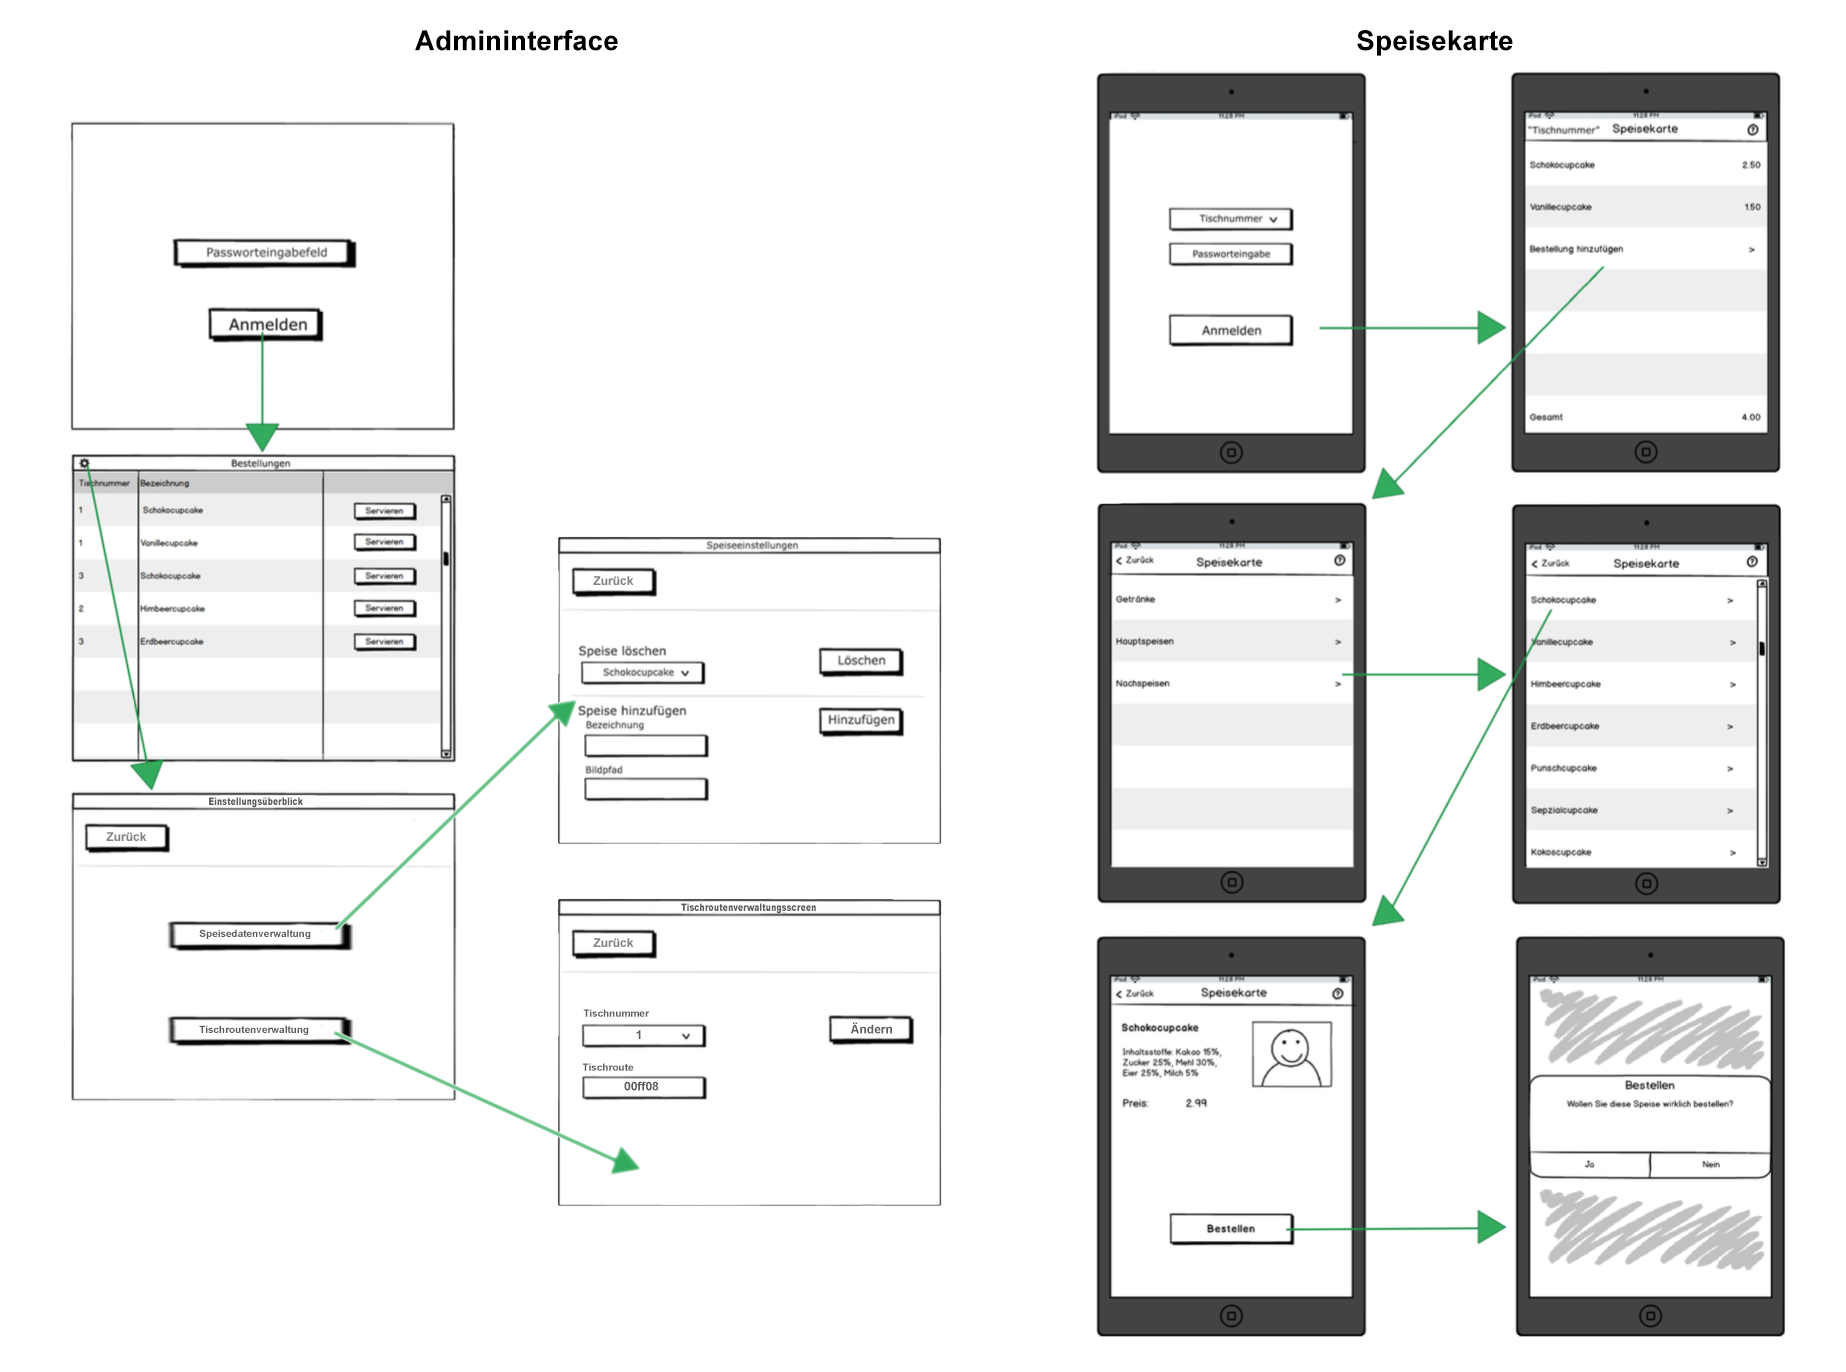
\includegraphics[width = 0.8\textwidth]{Bilder/Jok_alte_mockups}
			\par\end{centering}
			\caption{alte Mockups - Speisekarte}
			\label{alte Mockups - Speisekarte}
			\end{figure}\textbf{Admininterface}\\
			\begin{figure}[H]
			\begin{centering}
			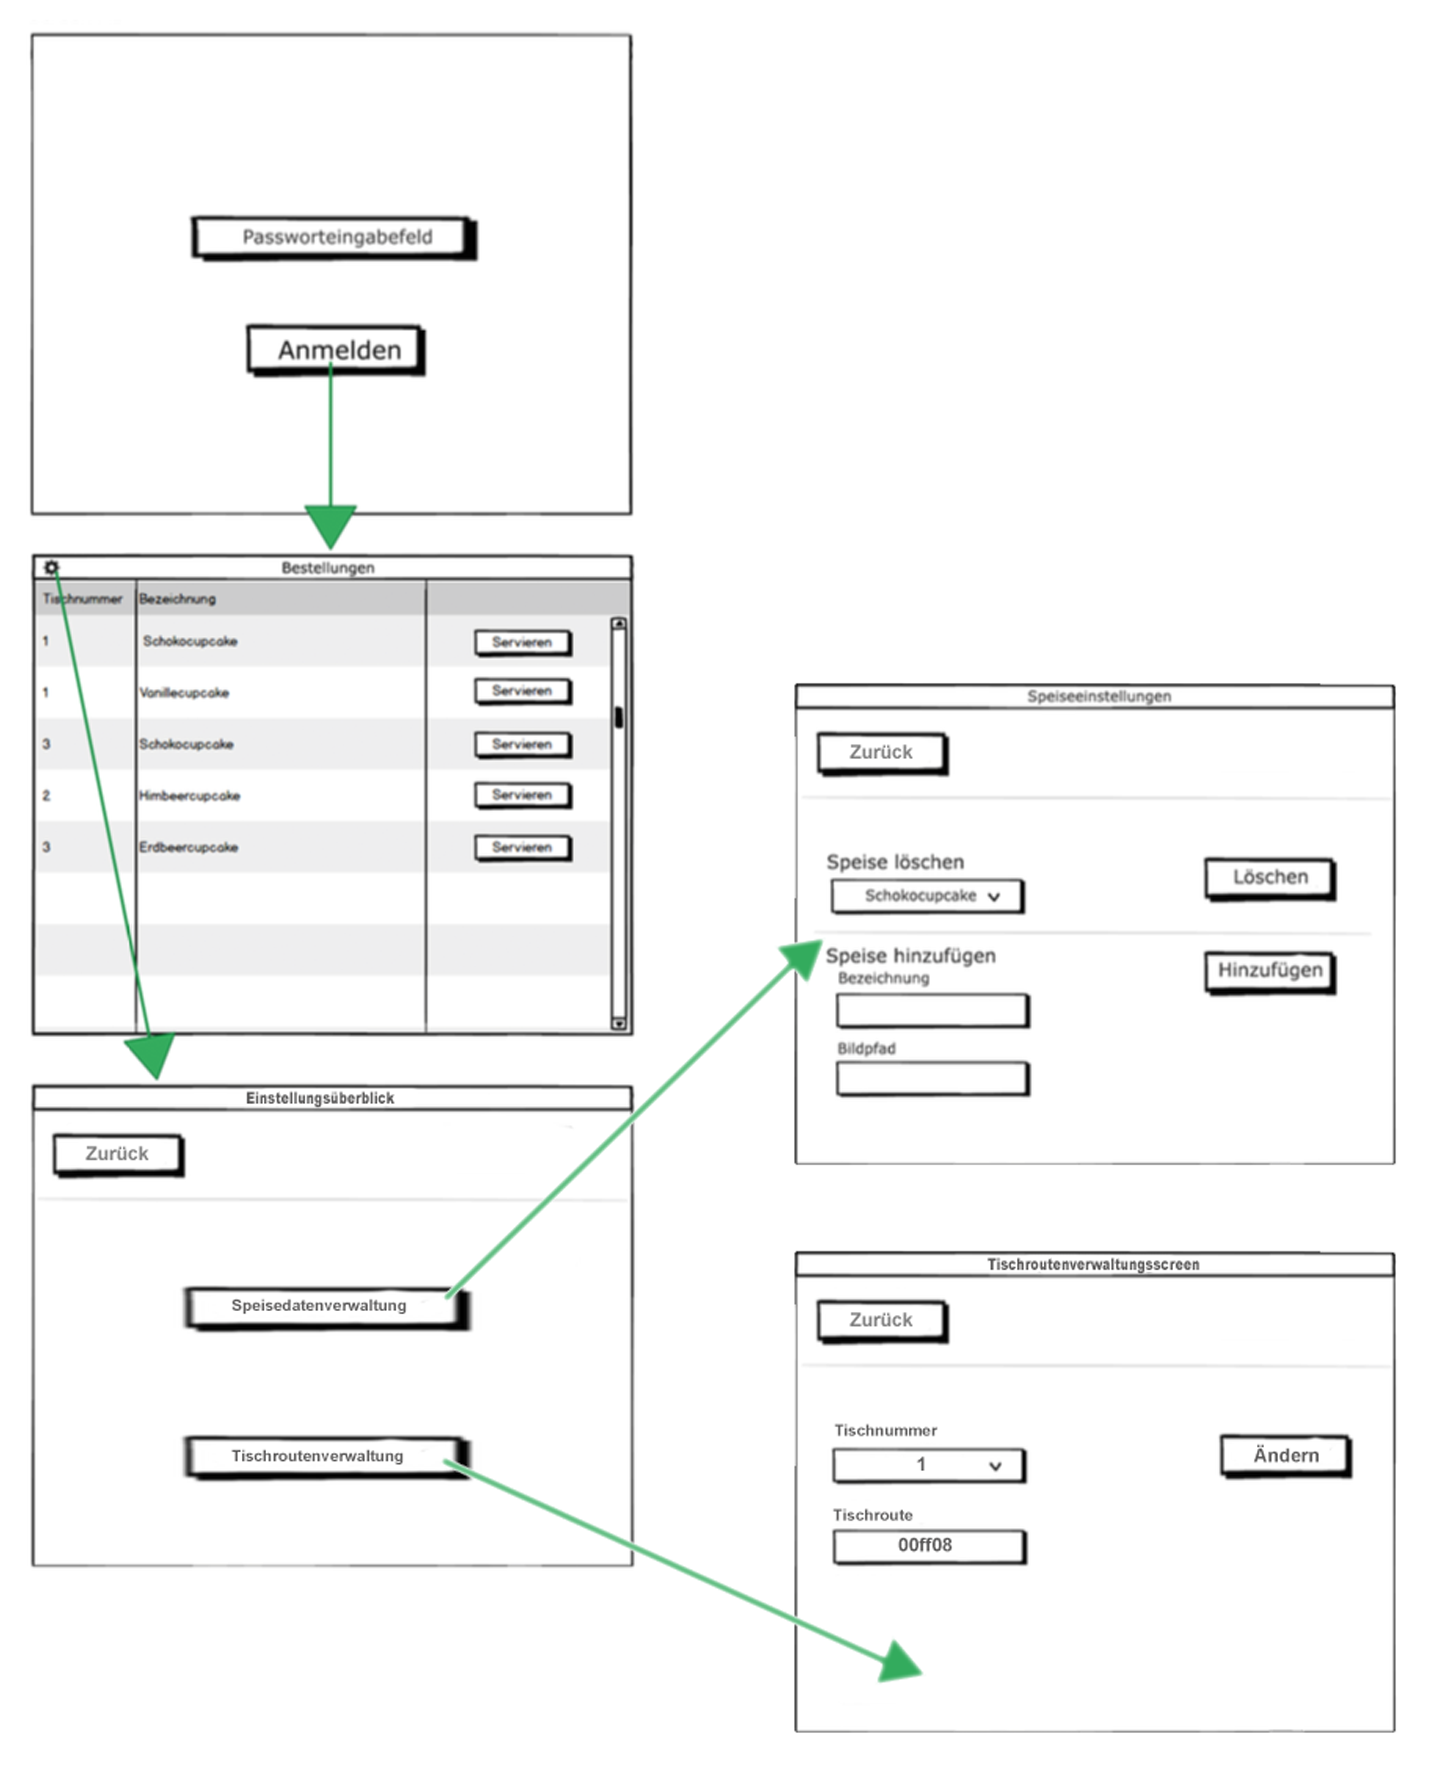
\includegraphics[width = 0.8\textwidth]{Bilder/Jok_alte_mockups_admin}
			\par\end{centering}
			\caption{alte Mockups - Admininterface}
			\label{alte Mockups}
			\end{figure}Während der Umsetzungsphase wurde jedoch realisiert, dass dies nicht sehr anwenderfreundlich ist. Daher wurde ein neues Konzept entwickelt, welches dem Gast die Möglichkeit bietet im Header jederzeit die Kategorie zu wechseln ohne den Screen verlassen zu müssen. Das Konzept des Admininterfaces wurde im Laufe der Zeit ebenfalls etwas überarbeitet. Beispielsweise wurde eine Alert-Box auf dem Hauptscreen eingefügt, um den Verbindungsstatus zwischen dem Hexacopter und dem Server anzuzeigen.
\\ \\
\textbf{neue Mockups}\\
\textbf{Speisekarte}\\
			\begin{figure}[H]
			\begin{centering}
			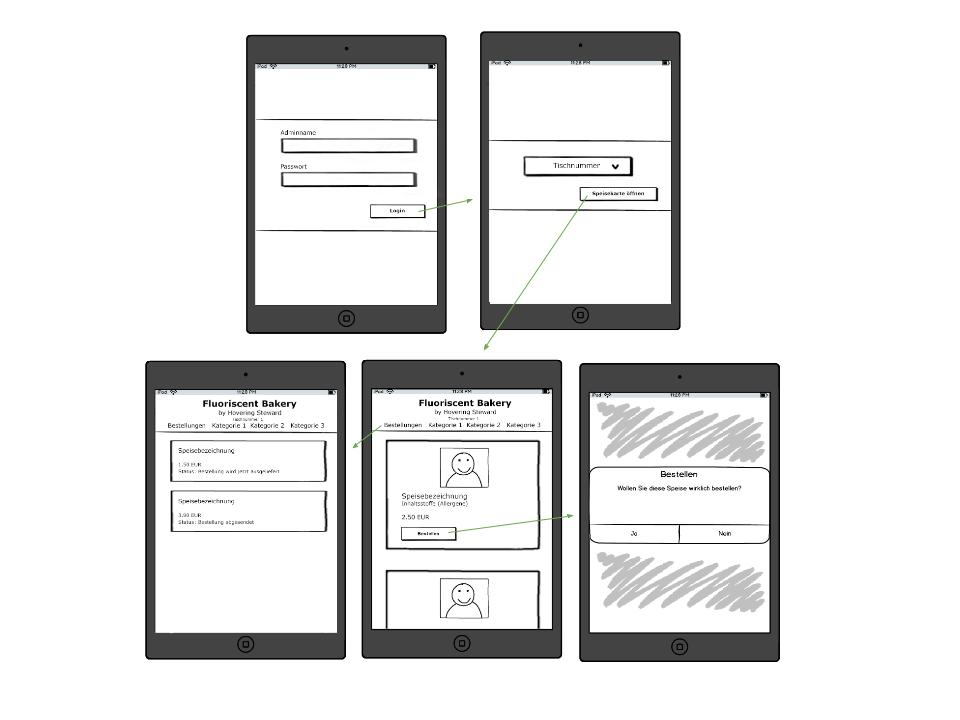
\includegraphics[width = 1\textwidth]{Bilder/Jok_neue_mockups}
			\par\end{centering}
			\caption{neue Mockups - Speisekarte}
			\label{neue Mockups - Speisekarte}
			\end{figure}\textbf{Admininterface}\\
			\begin{figure}[H]
			\begin{centering}
			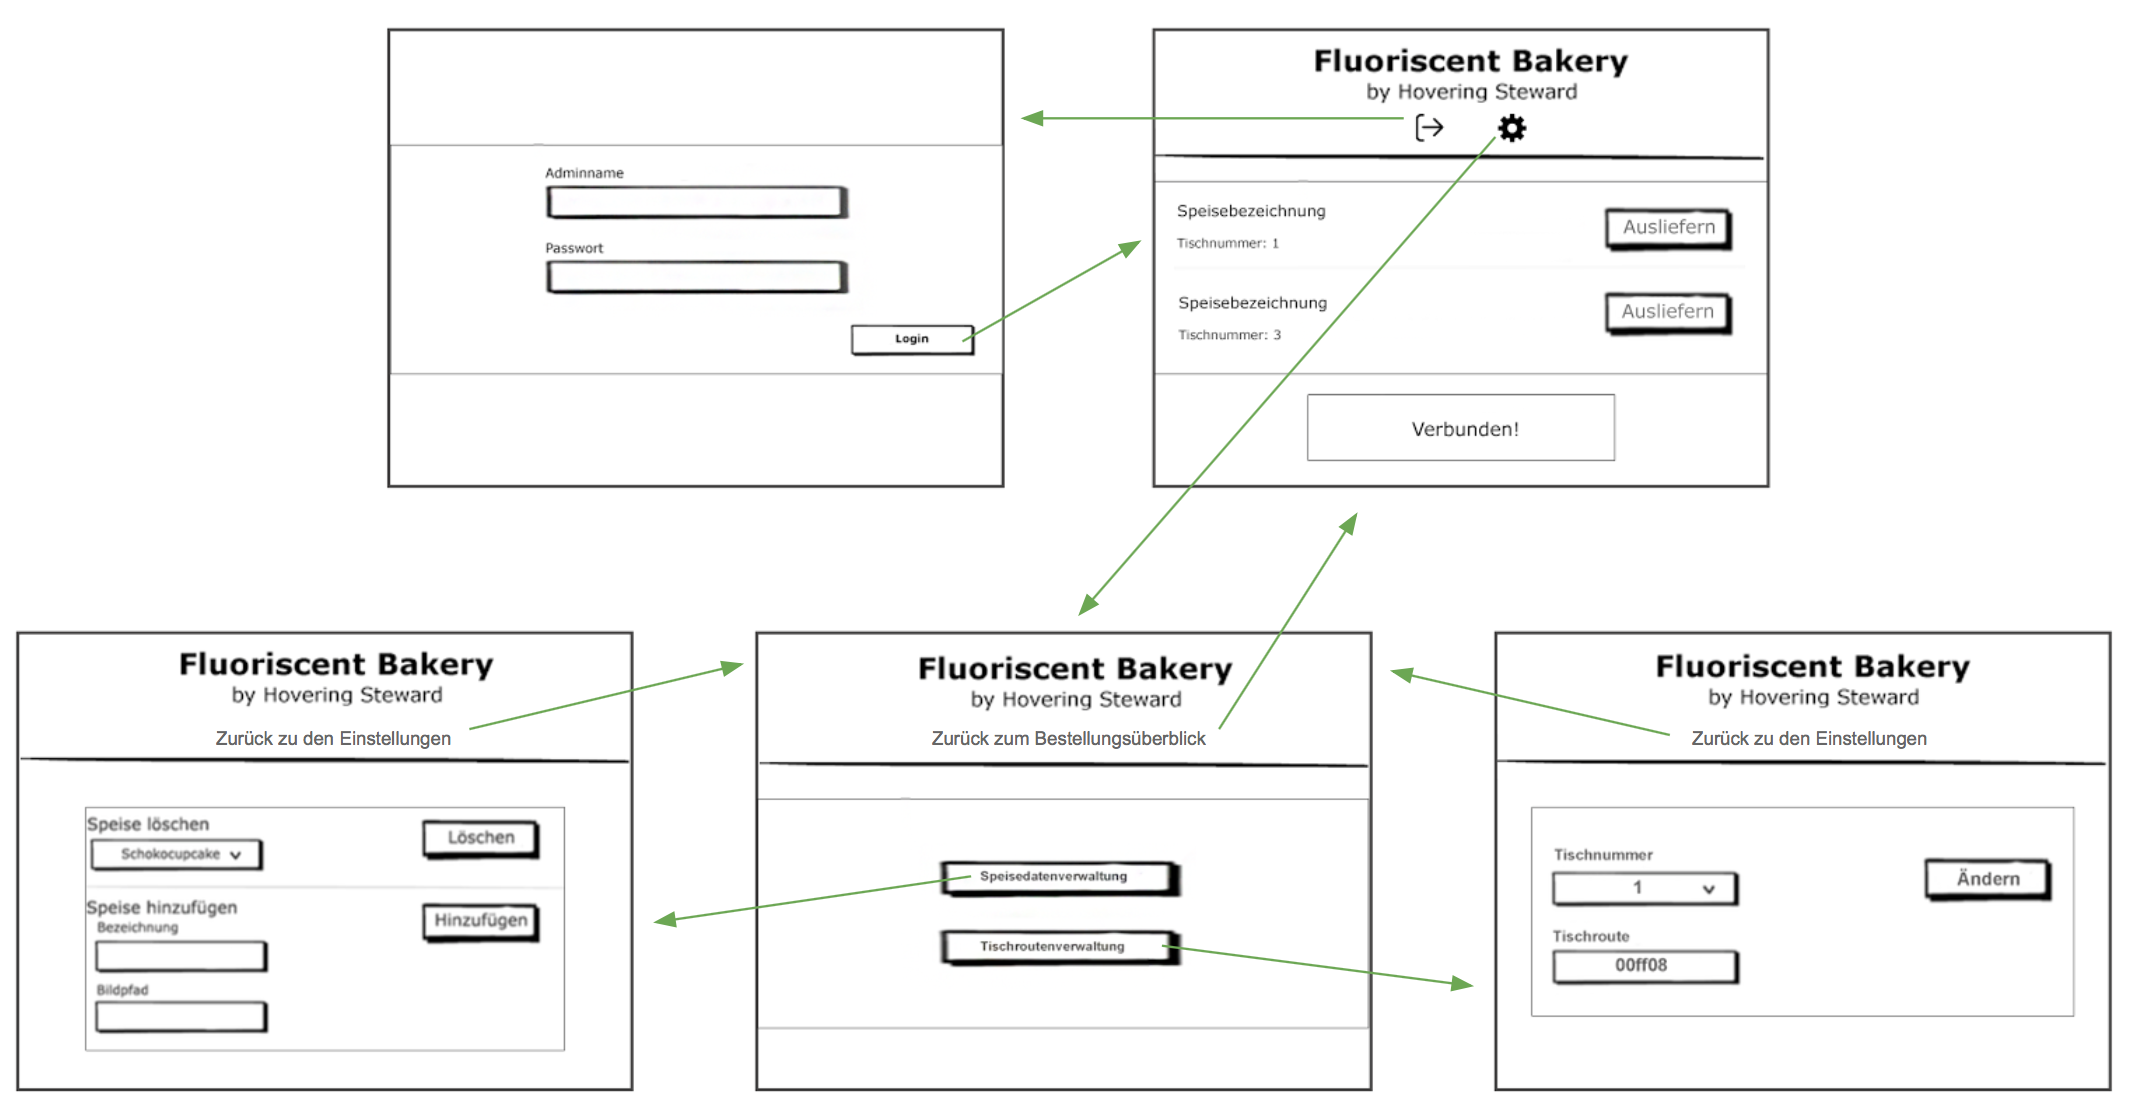
\includegraphics[width = 1\textwidth]{Bilder/Jok_neue_mockups_admin}
			\par\end{centering}
			\caption{neue Mockups - Admininterface}
			\label{neue Mockups - Admininterface}
			\end{figure}\textbf{Funktionalitäten der Applikation}\\
Wie an den Mockups bereits erkannt werden kann, wurde damals schon festgelegt welche Funktionalitäten die einzelnen Screens haben.
Diese sind, wie in den neuen Mockups festgelegt, folgende:\\ \\
\textbf{Funktionalitäten der digitalen Speisekarte}
\begin{itemize}
    \item \textbf{Loginscreen}\\
Der Loginscreen beeinhaltet sowohl ein Eingabefeld für den Administratornamen als auch für das Administratorpasswort und einen Loginbutton.
Falls die Anmeldedaten falsch eingegeben werden, wird eine Fehlermeldung in rot angezeigt, die den Admin darauf hinweist, dass die Anmeldedaten falsch eingegeben wurden.
Wenn das Anmeldeformular richtig ausgefüllt wurde, wird der Tischnummernauswahlscreen geöffnet.
    \item \textbf{Tischnummernauswahlscreen}\\
Auf diesem Screen befinden sich ein Dropdownmenü in welchem die Tischnummern zur Auswahl angezeigt werden und ein Button mit dem Label "Speisekarte öffnen". Nachdem auf diesen Button geklickt wurde, öffnet sich die Speisekarte mit dem Parameter der ausgewählten Tischnummer.
    \item \textbf{Speisekartenscreen}\\
Auf dem Speisekartenscreen kann sich der Gast oben im Header sowohl durch die Kategorien klicken, als auch seine bisher getätigten Bestellungen einsehen.
Sobald auf eine Kategorie geklickt wird, werden die dazugehörigen Speiseeinträge samt Informationen angezeigt. Zu jedem Speiseeintrag gibt es einen Bestellbutton.
Nachdem der Gast auf einen Bestellbutton klickt, öffnet sich eine Alertbox, welche ihn fragt ob er die ausgewählte Speise kostenpflichtig bestellen möchte. Falls der Anwender auf "Nein" klickt, kommt eine Meldung, dass der Bestellvorgang abgebrochen wird.
Wenn der Gast jedoch auf "Ja" klickt, öffnet sich eine Meldung, die ihn darauf hinweist, dass die Bestellung getätigt wurde. Anschließend kann er sie unter dem Menüpunkt "Bestellungen" ansehen und dort ihren aktuellen Status verfolgen.\\

  \end{itemize}
\textbf{Funktionalitäten des Adminbereichs}
\begin{itemize}
    \item \textbf{Loginscreen}\\
Der Loginscreen des Admininterface hat nahezu dieselben Funktionalitäten wie der, der digitalen Speisekarte. Der einzige Unterschied besteht darin, dass sich nach dem Klick auf den Loginbutton der Hauptscreen des Admininterfaces öffnet.
    \item \textbf{Hauptscreen}\\
Der Hauptscreen des Admininterfaces bietet in einer Liste den Überblick über alle Bestellungen, die noch nicht serviert wurden.
Neben jedem Bestelleintrag gibt es einen "Ausliefern"-Button. Sobald auf diesen geklickt wird, ändert sich der Tinyint-"ausliefern"-Wert in der Datenbank, damit das Javaprogramm weiß, von welcher Bestellung die Tischdaten an den Hexacopter geschickt werden sollen.
Im Header befindet sich ein Button mit einem Ausloggen-Symbol, damit der Administrator sich jederzeit abmelden kann. Weiters befindet sich im Header ein Button mit einem Einstellungssymbol, welches auf den Einstellungsübersichts-Screen verlinkt.
Unter der Bestelleintragliste wird eine Alert-Box angezeigt, welche den derzeitigen Verbindungsstatus zum Server anzeigt. Diese erscheint grün, falls die Verbindung steht, und rot sobald, die Verbindung abgebrochen ist.

    \item \textbf{Einstellungsübersicht-Screen}\\
Der Einstellungsübersichtsscreen verweist in einer div-Box mit zwei Buttons auf den Tischverwaltungsscreen und den Speise- und Kategorienverwaltungsscreen.
Oben im Header ermöglicht er es dem Admin wieder zurück zum Hauptscreen navigieren zu können.
    \item \textbf{Tischdatenverwaltungsscreen}\\
Der Tischdatenverwaltungsscreen bietet die Möglichkeit an die Tischroute der Tische zu verändern. Hierfür muss im Dropdownmenü eine Tischnummer ausgewählt werden, im Eingabefeld die neue Tischroute angegeben werden und anschließend auf den "Änderungen übernehmen"-Button geklickt werden.
    \item \textbf{Speise- und Kategorienverwaltungsscreen}\\
Im Speise- und Kategorienverwaltungsscreen können neue Speiseinträge und Kategorien erstellt als auch alte gelöscht werden.
Hierfür muss der Admin das jeweilige Formular ausfüllen und anschließend auf den dazugehörigen Submit Button klicken.
  \end{itemize}
  \subsection{Umsetzung}

    \subsubsection{Layout}

Zu Beginn der Umsetzung des Layouts wurde der Package Manager Bower mithilfe des Befehls "npm install -g bower" global über das Terminal installiert, damit im weiteren Vorgehen die benötigten Pakete verwaltet werden konnten. Alle relevanten Informationen, der zu verwaltenden Pakete werden mithilfe dieses Managers in der Datei "bower.json" dokumentiert, welche mit folgenden Kommandozeileneingaben generiert wurde:
	\lstset{language = bash}
  	\begin{lstlisting}
  	bower init
  	\end{lstlisting}
Nachdem Bower in dem Projektverzeichnis installiert wurde, konnten alle notwendigen Bibliotheken über das Terminal installiert werden. Außerdem wurden die Abhängigkeiten in der Bower-Datei festgelegt. Dies war vor allem für "Bootstrap 4 alpha" wichtig, da es sonst nicht möglich gewesen wäre die neueste Version zu verwenden. Die Bibliothek jQuery wurde automatisch mitinstalliert, da Bootstrap als Abhängigkeit definiert wurde. Für die Installation von Gulp wurden einige weitere Bibliotheken benötigt, welche mithilfe von Bower einfach heruntergeladen werden konnten.
Durch die Kombination von Bootstrap und Sass konnten die Bootstrap Style-Attribute, welche in den herkömmlichen Bootstrapklassen verwendet werden, in der Sass-Datei wie Variablen behandelt werden. Das bedeutet, dass beispielsweise die Schriftart mit der Zuweisung einer einzigen Variable sogleich für alle Seiten übernommen wurde.
	\lstset{language = html}
  	\begin{lstlisting}
  	$font-family-sans-serif:	'PT Sans', sans-serif;
  	\end{lstlisting}
Für das Streaming Build System Gulp wurde eine Javascript-Datei generiert. In dieser wurde die Sass-Datei kompiliert und festgelegt, dass diese laufend beobachtet werden soll, sobald der Gulp-Befehl im Terminal eingegeben wird. Außerdem wurden die jQuery und Bootstrap Javascript-Dateien mithilfe von Gulp minimiert und miteinander verkettet, damit nur ein einziges File in den jeweiligen Screens eingebunden werden musste.
Nachdem die dadurch generierte CSS-Datei, im Header der Template-Files aufgerufen wurde, konnten die Bootstrap Klassen verwendet werden, indem sie in den class-Attributen der jeweiligen Elemente deklariert wurden.
Für den Aufbau der Screens wurden drei verschiedene Grundkonzepte angwendet:
\begin{itemize}
    \item \textbf{Loginscreens und Tischnummernauswahl-Screen}\\
Für diese Screens wurde lediglich eine div-Box benötigt, welche sich in der Mitte des Screens befindet. Ihre Seitenränder grenzen an die des Bildschirms. Der Inhalt dieser Box besteht aus dem Anmelde- und Auswahlformular.
	\item \textbf{Speisekarten und Einstellungsscreens}\\
Bei diesen Screens wurde ein Header angezeigt, in welchem sowohl der Titel der Veranstaltung, für welche die Applikation benötigt wird, als auch der Name der Herrsteller angegeben wird. Dieser befindet sich ganz oben auf dem Screen. Unter dem Titel befinden sich die Navigationsbuttons, welche auf andere Screens verlinken. Der Hauptinhalt wird von weiteren div-Boxen gebildet, in welchen sich die einzelnen Speiseeinträge und Einstellungsformulare befinden.
    \item \textbf{Hauptscreen des Admininterfaces}\\
Der Hauptscreen enthält ebenfalls einen Header, mit nahezu demselben Schema wie bei der Speisekarte. Der einzige Unterschied liegt darin, dass sich die Navigationsbuttons bei diesem Screen links und rechts vom Titel in Form von Icons befinden. Die Bestellungen werden als Liste dargestellt. Unter dieser Liste wird der Verbindungsstatus vom Hexacopter zum Server in einer Alert-Box angezeigt.
  \end{itemize}
Das Design der Screens ist dem des Blogs sehr ähnlich, da diese aneinander angepasst wurden. Der Hintergund besteht daher ebenfalls aus einem Tisch, der den Esstisch symbolisieren soll. Die Inhalte werden jeweils in leicht durchsichtigen weißen div-Boxen angezeigt. Dieses Layout ist absichtlich nicht sehr aufwendig gestaltet, damit es elegant und modern auf den Anwender wirkt.
Um dem Gast die Speisen schmackhaft zu machen, werden sie anhand von Fotos visuell dargestellt.
Das finale Layout der Screens sieht daher folgendermaßen aus:\\
\\
\textbf{Screens der digitalen Speisekarte}
			\begin{figure}[H]
			\begin{centering}
			\fbox{ 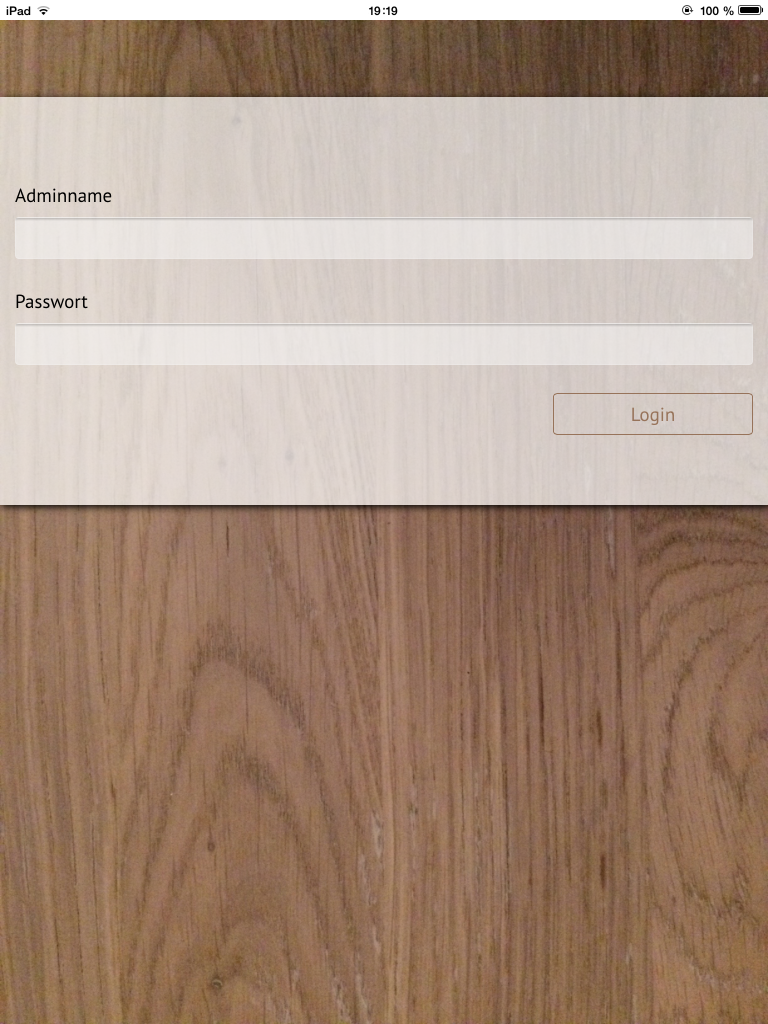
\includegraphics[width = 0.45\textwidth]{Bilder/Jok_login} }
			\fbox{ 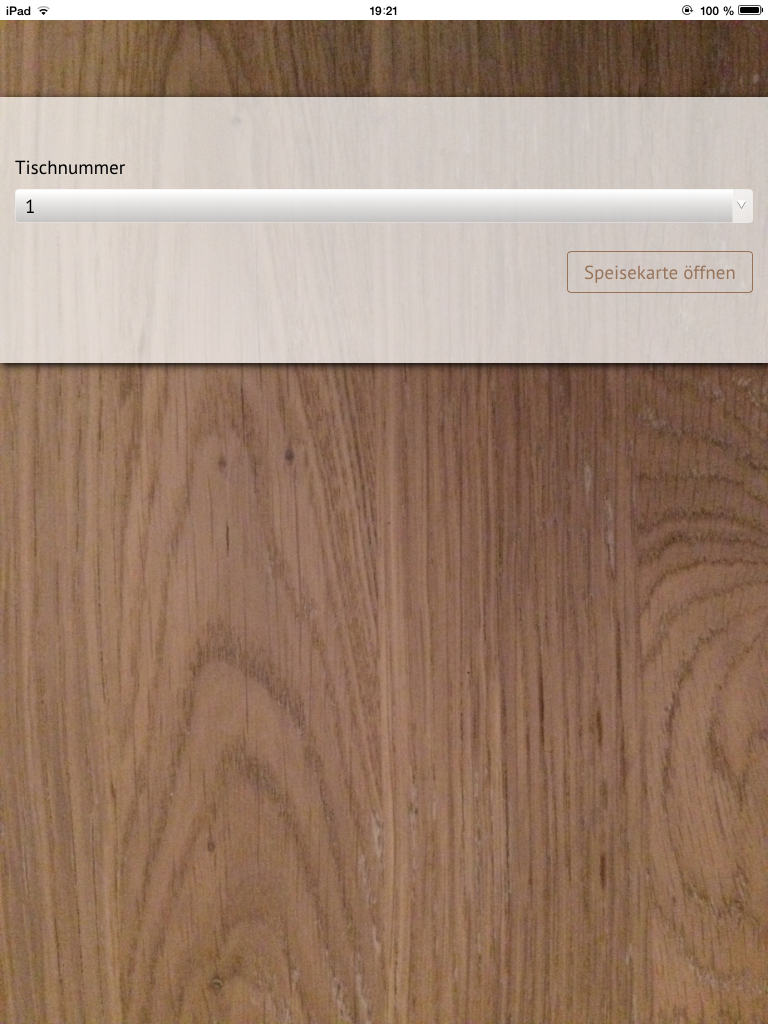
\includegraphics[width = 0.45\textwidth]{Bilder/Jok_tnr} }
			\par\end{centering}
			\caption{Screens: Loginscreen / Tischnummernauswahl}
			\label{Screens: Loginscreen / Tischnummernauswahl}
			\end{figure}

			\begin{figure}[H]
			\begin{centering}
			\fbox{ 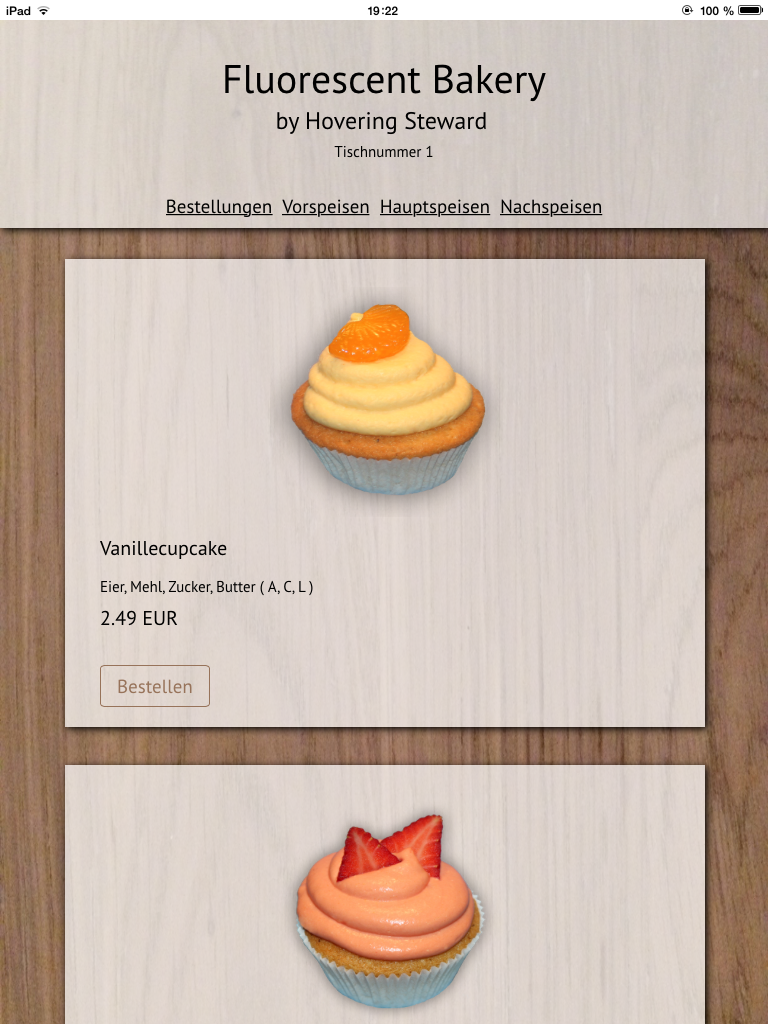
\includegraphics[width = 0.45\textwidth]{Bilder/Jok_speisekarte} }
			\fbox{ 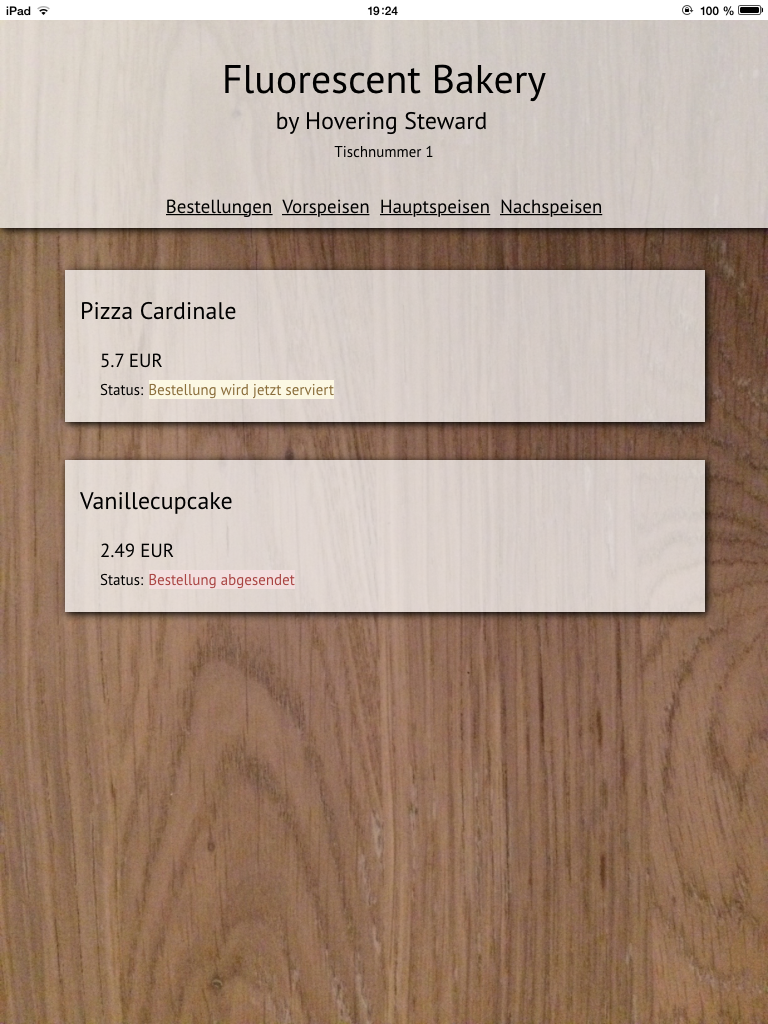
\includegraphics[width = 0.45\textwidth]{Bilder/Jok_status} }
			\par\end{centering}
			\caption{Screens: Speisekarte / Bestellungsüberblick}
			\label{Screens: Speisekarte / Bestellungsüberblick}
			\end{figure}
\textbf{Screens des Admininterfaces}
			\begin{figure}[H]
			\begin{centering}
			\includegraphics[width = 0.9\textwidth]{Bilder/Jok_admin_login}
			\par\end{centering}
			\caption{Screen - Login}
			\label{Screen - Login}
			\end{figure}
			\begin{figure}[H]
			\begin{centering}
			\includegraphics[width = 0.9\textwidth]{Bilder/Jok_admin_hauptscreen}
			\par\end{centering}
			\caption{Screen: Hauptscreen}
			\label{Screen: Hauptscreen}
			\end{figure}
			\begin{figure}[H]
			\begin{centering}
			\includegraphics[width = 0.9\textwidth]{Bilder/Jok_admin_einstellungsueberblick}
			\par\end{centering}
			\caption{Screen: Einstellungsüberblick}
			\label{Screen: Einstellungsüberblick}
			\end{figure}
			\begin{figure}[H]
			\begin{centering}
			\includegraphics[width = 0.9\textwidth]{Bilder/Jok_admin_speiseverwaltung}
			\par\end{centering}
			\caption{Screen: Speise- und Kategorieverwaltung}
			\label{Screen: Speise- und Kategorieverwaltung}
			\end{figure}
			\begin{figure}[H]
			\begin{centering}
			\includegraphics[width = 0.9\textwidth]{Bilder/Jok_admin_tischdaten}
			\par\end{centering}
			\caption{Screen: Tischdatenverwaltung}
			\label{Screen: Tischdatenverwaltung}
			\end{figure}
    \subsubsection{Datenausgabe}

Wie bereits zuvor erwähnt wurde, ermöglicht die Template Engine Twig einen vereinfachten Zugriff auf die Variablen, welche vom Controller übergeben wurden. Um eine einzige Variable aufzurufen, musste diese lediglich mit zwei geschwungenen Klammern umhüllt werden.
\lstset{language = php}
  	\begin{lstlisting}
{{ VARIABLEN_BEZEICHNUNG }}
\end{lstlisting}
Hierbei kann über den beliebig gewählten Namen, welchen man beim Rückgabewert der Action-Funktion mitgeliefert hat, auf die Variable zugegriffen werden.
Falls die Variable mit einem herkömmlichen String verbunden werden soll, wird eine Tilde als Verknüpfungszeichen benötigt.
\lstset{language = php}
  	\begin{lstlisting}
var STRING_BEZEICHNUNG= {{ VARIABLEN_BEZEICHNUNG }}~"TEXT";
	\end{lstlisting}
Die Variable kann allerdings auch problemlos in einer von Twig zur Verfügung gestellten IF-Anweisung verwendet werden.
Um die Datenbankdaten der digitalen Speisekarte auslesen zu können, wurde die von Twig mitgelieferte Art Schleifen zu generieren verwendet. Damit die Tabellenspalten einzeln angezeigt werden konnten, musste an die Bezeichnung des aktuellen Tabelleneintrags einfach die Spaltenbezeichnung angehängt werden.
\lstset{language = php}
  	\begin{lstlisting}

	{{ AKTUELLER_TABELLENEINTRAG.SPALTEN_BEZEICHNUNG }}

	\end{lstlisting}
Falls eine Relation zu einer anderen Datenbanktabelle besteht, wie zum Beispiel beim Zugriff auf die Speiseeinträge der jeweiligen Kategorien, musste im Aufruf ebenfalls auf diese verwiesen werden, bevor der auszugebende Wert von ihr geholt werden konnte.
\lstset{language = php}
  	\begin{lstlisting}

{{ AKTUELLER_TABELLENEINTRAG.VERLINKTE_TABELLE.SPALTENBEZEICHNUNG }}

	\end{lstlisting}
Bei Werten, welche auf diese Art und Weise von der Datenbank geholt werden, wurde darauf geachtet, dass sie kompatibel für Textausgaben kodiert wurden. Dies wird am besten mit einer JSON-Kodierung bewerkstelligt.
\lstset{language = php}
  	\begin{lstlisting}
var VARIABLEN_BEZEICHNUNG =
{{ AKTUELLER_TABELLENEINTRAG.SPALTENBEZEICHNUNG|json_encode|raw  }};
	\end{lstlisting}
Mit diesem Schema konnten alle Speisekarteninformationen in dem Frontend der Applikation angezeigt werden.

    \subsubsection{Formulargenerierung}

Um das Formular, welches über den Controller übermittelt wurde, anzeigen zu können, musste in der Twig-Datei nicht mehr viel erledigt werden. Hier galt es nur noch, die bereits definierten Eingabefelder aufzurufen und ihnen nach Belieben Attribute zuzuteilen.
\lstset{language = java}
  	\begin{lstlisting}
{{ form_start(FORMULAR_BEZEICHNUNG) }}
            {{ form_label(FORMULAR_BEZEICHNUNG.FORMULARFELD_BEZEICHNUNG}}
            {{ form_widget(FORMULAR_BEZEICHNUNG.FORMULARFELD_BEZEICHNUNG,
            {'attr': {'ATTRIBUT_BEZEICHNUNG': 'ATTRIBUT_WERT'}}) }}
{{ form_end(FORMULAR_BEZEICHNUNG) }}
	\end{lstlisting}
Um dem Template mitzuteilen, dass die Generierung eines Formulars gestartet werden soll, musste die "start()"-Funktion aufgerufen und ihr die Bezeichnung des Formulars, welche im Rückgabewert der Actionfunktion im Controller definiert wurde, als Parameter mitgeschickt werden.
Anschließend kann auf alle Felder und Labels des Formulars zugegriffen werden. Es empfiehlt sich zuerst das Label mit der "label()"-Methode, welche sowohl die Bezeichnung des Formulars als auch die des Eingabefelds übergeben werden sollen, und anschließend erst das Eingabefeld mit der "widget()"-Funktion, der dieselben Parameter übermittelt werden sollen, abzurufen. Es gibt die Möglichkeit jedem Label und Eingabefeld Attribute zuzuteilen um sie beliebig zu gestalten. Im Frontend werden alle Formularelemente gleich behandelt, da bereits im Controller die spezifischen Funktionalitäten zugewiesen wurden. Das heißt die Generierung eines Buttons in einer Twig-Datei unterscheidet sich nicht von der eines Texteingabefeldes.
Mit diesem Codeschema wurden alle Login-, Speisen- und Tischdatenverwaltungsformulare visuell dargestellt.

  \subsection{Herausforderungen und Lösungen}

\textbf{Apache Zugriffsverweigerung}\\
Damit die Applikation über den Apache HTTP Server im Frontend angezeigt werden kann, musste in der "app.php"-Datei angegeben werden, dass die digitale Speisekarte auch in einer Produktionsumgebung, also auch im gewerblichen Gebrauch, aufgerufen werden kann und nicht nur der Symfony-Server darauf Zugriff hat.
	\lstset{language=php}
  	\begin{lstlisting}
$kernel = newAppKernel('prod', true);
  	\end{lstlisting}
Der Wert "prod" steht hierbei für "production environment", also für die Produktionsumgebung.

\section{Testphase}
Für die Testphase wurden präzise Testfälle erstellt, welche abgesehen von TC-5 von einer externen Person getestet wurden.

\begin{table}[H]
\centering
\begin{tabular}{|p{0.5cm}|p{3cm}|p{4.5cm}|p{4cm}|p{2cm}|}
\hline \textbf{ID} & \textbf{Bezeichnung} & \textbf{Testszenario} & \textbf{Erwartetes Ergebnis} & \textbf{Ergebnis erreicht?} \\\hline
\hline 1 & Adminlogin & Admin meldet sich mit \newline richtigen Anmeldedaten \newline an & Hauptscreen des \newline Admininterfaces wird \newline angezeigt & Ja \\\hline
\hline 2 & Speisebestellung & eine Speise wird bestellt & neuer Bestellungseintrag wird erstellt und in \newline Bestellliste angezeigt & Ja \\\hline
\hline 3 & "Ausliefern"-Wert \newline ändern & Admin klickt auf "Ausliefern"-Button & "ausliefern"-Wert der Speise wird auf 1 gesetzt & Ja \\\hline
\hline 4 & Tischroute \newline schicken & Hexacopter schickt \newline bestimmte Nachricht an Server & Server schickt \newline Tischnummer zurück & Ja \\\hline
\hline 5 & Speiseeintrag \newline hinzufügen & Admin gibt neue \newline Speisedaten ins Formular ein und klickt auf \newline "Speiseeintrag hinzufügen" & neuer Speiseeintrag wird in Datenbank angelegt & Ja \\\hline
\hline 6 & Kategorie \newline hinzufügen & Admin gibt neue \newline Kategoriebezeichnung ins \newline Formular ein und klickt auf \newline "Kategorie hinzufügen” & neue Kategorie wird in Datenbank angelegt & Ja \\\hline
\hline 7 & Speiseeintrag \newline löschen & Admin wählt Speiseeintrag aus und klickt auf "Speiseeintrag Löschen"-Button & ausgewählter \newline Speiseeintrag wird \newline gelöscht & Ja \\\hline
\hline 8 & Kategorie \newline löschen & Admin wählt Kategorie aus und klickt auf "Kategorie Löschen"-Button & ausgewählte Kategorie wird gelöscht & Ja \\\hline
\hline 9 & Tischroute \newline verändern & Admin wählt Tischnummer aus und gibt Tischroute ins Formularfeld ein & Tischroute des Tisches wird geändert & Ja \\\hline
\end{tabular}
\caption{Testfälle der Applikation und des Java Programms}
\end{table}

\section{Persönliche Erfahrungen}
Da ich zuvor kaum mit einer der hierfür verwendeten Technologien gearbeitet habe, konnte ich mir dank der Diplomarbeit einige neue Fähigkeiten erlernen.
Zwar habe ich bereits in der vierten Klasse die Grundlagen eines MVC-Frameworks gelernt, doch war mir damals trotzdem kaum klar, wie es genau funktioniert und wie viele positive Eigenschaften es eigentlich mit sich bringt.
Zuerst dachte ich, dass es mehr Aufwand mit sich bringen würde, da ich mich nicht gut damit auskannte, doch mittlerweile ist die Verwendung von Symfony für mich kaum noch wegzudenken. Ohne diesem Framework, hätte ich mich vermutlich kaum in meiner Codestruktur zurechtgefunden.
So ging es mir jedoch nicht nur mit Symfony sondern nahezu mit jeder anderen Technologie die verwendet wurde auch.
Ich habe zwar ziemlich viel Zeit dafür aufgebracht mit Doctrine zurechtzukommen, doch dies hat sich auf jeden Fall ausgezahlt. Dadurch konnte ich nämlich Änderungen in der Datenbank ohne großen Aufwand vornehmen.
Ich bin wirklich froh darüber, dass ich mit der Template Engine Twig gearbeitet habe, da ich dadurch keinen aufwendigen Code in den Dateien für die visuelle Darstellung zur Ausgabe von Variablen eingeben musste, sondern lediglich wenige Zeilen mit dem Twig-Syntax angeben konnte.
\\
Dadurch, dass wir uns im Projektteam zu Beginn der Diplomarbeit kaum kannten, führten wir Coachings ein, welche regelmäßig stattfanden. In diesen wurde der Fokus neben der Planung des Projekts auch immer wieder auf das Zusammenschweißen der Teammitglieder gelegt. Dadurch kann ich mittlerweile wirklich behaupten, dass wir fünf uns nun prima miteinander verstehen und auch längere Zeit miteinander auskommen ohne dass es zu Streitigkeiten kommt. Wir können alle offen miteinander über Probleme reden und uns darauf verlassen, dass jeder dem anderen bei Schwierigkeiten mit Rat oder Motivation zur Seite steht.
\\
Mein persönliches Fazit ist, dass ich dank dieser Diplomarbeit meinen Wissenshorizont um ein Vielfaches erweitert habe und auch, dass meine sozialen Kompetenzen davon profitiert haben.

\section{Ergebnisse}
Sowohl die Screens der digitalen Speisekarte als auch die des Admininterfaces sind funktionstüchtig.
Das Java Programm bietet ebenfalls wie im optionalen Ziel definiert, die Möglichkeit die Tischroute automatisch an den Hexacopter schicken zu können.
